%
% FH Technikum Wien
% !TEX encoding = UTF-8 Unicode
%

\documentclass[Bachelor, BMR, ngerman]{twbook}
\usepackage[utf8]{inputenc}
\usepackage[T1]{fontenc}


% --------------------------------------------------
% CITE
% --------------------------------------------------
\newcommand{\FHTWCitationType}{HARVARD} 
\ifthenelse{\equal{\FHTWCitationType}{HARVARD}}{\usepackage{harvard}}{\usepackage{bibgerm}}


% --------------------------------------------------
% FORMAT CODE LISTINGS
% --------------------------------------------------
\usepackage[final]{listings}
\lstset{captionpos=b, numberbychapter=false,caption=\lstname,frame=single, numbers=left, stepnumber=1, numbersep=2pt, xleftmargin=15pt, framexleftmargin=15pt, numberstyle=\tiny, tabsize=3, columns=fixed, basicstyle={\fontfamily{pcr}\selectfont\footnotesize}, keywordstyle=\bfseries, commentstyle={\color[gray]{0.33}\itshape}, stringstyle=\color[gray]{0.25}, breaklines, breakatwhitespace, breakautoindent}
\lstloadlanguages{[ANSI]C, C++, [gnu]make, gnuplot, Matlab}
\makeatletter
\providecommand\listacroname{}
\@ifclasswith{twbook}{english}
{%
    \renewcommand\lstlistingname{Code}
    \renewcommand\lstlistlistingname{List of Code}
    \renewcommand\listacroname{List of Abbreviations}
}{%
    \renewcommand\lstlistingname{Quellcode}
    \renewcommand\lstlistlistingname{Quellcodeverzeichnis}
    \renewcommand\listacroname{Abkürzungsverzeichnis}
}
\newcommand\listoflolentryname\lstlistingname
\makeatother
\newcommand{\listofcode}{\phantomsection\lstlistoflistings}


% --------------------------------------------------
%  AUXILARY PACKAGES
% --------------------------------------------------
\usepackage{blindtext}
\usepackage{esvect} % Vektorpfeile
\usepackage{textcomp}
\usepackage{float} % Positionierung (H)


% --------------------------------------------------
%  TABLE PACKAGES
% --------------------------------------------------
\usepackage{colortbl} % Farbe
\usepackage{tabularx} % Zeilenumbruch (lädt auch pkg: array) 
\newcolumntype{C}[1]{>{\centering\arraybackslash}p{#1}}


% --------------------------------------------------
%  MATH PACKAGES
% --------------------------------------------------
\usepackage{amsmath}
\usepackage{relsize}
\usepackage{tocloft} % Formelverzeichnis


% --------------------------------------------------
% GRAPHIC PACKAGES
% --------------------------------------------------
\usepackage{graphicx}
\usepackage[export]{adjustbox}
\graphicspath{ {./Images/} }

\usepackage{svg}
\usepackage{calc}
\svgpath{ {./Images/} }


% --------------------------------------------------
% TIKZ PACKAGES
% --------------------------------------------------
\usepackage{tikz}
\usepackage{tikzscale}
\usetikzlibrary{babel}


\usetikzlibrary{angles, quotes, decorations.markings}


% --------------------------------------------------
% TITLE & AUTHOR
% --------------------------------------------------
\title{Auslegung und Konstruktion eines Delta-Roboters zur Untersuchung der inversen Kinematik}
\author{Felix Schausberger}
\studentnumber{mr16b049}
%\author{Titel Vorname Name, Titel\and{}Titel Vorname Name, Titel}
%\studentnumber{XXXXXXXXXXXXXXX\and{}XXXXXXXXXXXXXXX}
\supervisor{Mohamed Aburaia, MSc}
%\supervisor[Begutachter]{Titel Vorname Name, Titel}
%\supervisor[Begutachterin]{Titel Vorname Name, Titel}
%\secondsupervisor{Titel Vorname Name, Titel}
%\secondsupervisor[Begutachter]{Titel Vorname Name, Titel}
%\secondsupervisor[Begutachterinnen]{Titel Vorname Name, Titel}
\place{Wien}


% --------------------------------------------------
% KURZFASSUNG, ABSTRACT & KEYWORDS
% --------------------------------------------------
\kurzfassung{
    
    % Motivation
    % Stetig wachsender Einfluss technologiebezogener Industriebranchen machen den Erwerb technologischer Kompetenzen zu einem Schlüsselelement für den Erfolg künftiger Studentengenerationen.
    Stetig zunehmende Relevanz der Automatisierung in diversen Industriebranchen machen den Erwerb technologischer Kompetenzen zu einem Schlüsselelement für den Erfolg künftiger Studentengenerationen.
    %
    % Problem - und Aufgabenstellung
    Trotz Bestrebungen von Bildungsreformen versucht ein Großteil des derzeitigen Lehrsystems weiterhin, Auszubildende auf die Zukunft vorzubereiten, indem Methoden der Vergangenheit angewandt werden. Aktuellen Bildungslehrplänen fehlt es häufig an Möglichkeiten, Studierenden Wechselwirkungen zwischen einzelnen Ingenieursgebieten zu vermitteln. Folglich scheitern Auszubildende häufig daran,  fächerübergreifende Zusammenhänge und Abhängigkeiten herzustellen. Durch die Bereitstellung eines angemessenen Einstiegspunkts in die Konstruktion und Auslegung von Robotern könnte das vielseitige Feld angehenden Ingenieuren zugänglicher gemacht werden.
    %
    % Methoden
    Um dies zu erreichen wird als Lösungsansatz in der vorliegenden Arbeit die mechatronische Entwicklung eines Prototyps einer parallelkinematischen Maschine, eines Delta-Roboters, vorgestellt. Das System integriert anwendungsbezogen Wissen aus Mechanik, Elektrotechnik und Informatik. Um eine modulare Struktur zu ermöglichen wird der Aufbau mit ”smarten” Antrieben realisiert. Infolgedessen kann der Roboter bei Anforderungsänderung dynamisch konfiguriert werden, um individuell auf spezielle Aufgaben angepasst zu werden. Die verwendeten Antriebe erleichtern die Entwicklung von Robotern, da das System schnell und kostengünstig moduliert werden kann. Darüber hinaus werden, durch Kombination der modularen Hardware und Open-Source-Software, weder spezielles industrielles Equipment noch Forschungseinrichtungen benötigt, um praxisorientierte Lehrinhalte zu vermitteln und Forschungsmöglichkeiten zu bieten. 
    %
    % Zusammenfassung und Ergebnisse
    Die Ergebnisse zeigen, dass durch das Zusammenspiel dieser Vorteile ein Prototyp für didaktische Zwecke in der akademischen Ausbildung eigensicher, transportabel und kostengünstig hergestellt werden kann, um angehenden Ingenieuren die einzigartige Möglichkeit zu bieten, parallelkinematische Maschinen praxisorientiert zu studieren.

}
    
\schlagworte{

    Delta-Roboter, Parallelroboter, Modellierung von Robotern, Rekonfigurierbarer Roboter

}

\outline{

    % Motivation
    % The ever-increasing influence of industrial sectors makes the acquisition of technological competences a key element for the success of the next generations of students. 
    The ever-increasing influence of automation in various branches of industry makes the acquisition of technological competencies a key element for the success of future generations of students.
    %
    % Problem statement
    However, despite efforts to reform education, much of the current teaching system continues to prepare students for the future by using methods from the past. Current educational curricula often lack opportunities to provide interdependencies between individual areas of engineering. Trainees are often unable to establish connections between them. By providing an appropriate and approachable entry point, the versatile field of designing robotic systems could be made more accessible to aspiring engineers.
    %
    % Approach
    As an approach, in the present thesis, the development of a prototype of a parallel kinematic machine, a Delta-robot, is presented. The system integrates knowledge from mechanics, electrical engineering and computer science. To allow a modular structure, the entity is realized via ''smart'' drives. The robot can thus be dynamically changed upon request to be customized to specific tasks. The drives facilitate the development, as the robot can be modulated quickly and inexpensively. In addition, the modular hardware in combination with open source software does neither require any specialized industrial equipment nor research establishments to impart practice-oriented content and research opportunities. 
    %
    % Conclusion an results
    As a result, through the interaction of these advantages, a prototype for didactic purposes in academic education can be manufactured in an intrinsically safe, portable and cost-effective manner to give prospective engineers the unique opportunity of studying parallel kinematic machines in a practical way.

}

\keywords{

    Delta-Robot, Parallel robot, Robotic modeling, Reconfigurable robot

}

\acknowledgements{

    An dieser Stelle möchte ich mich bei allen bedanken, die mich während des Studiums begleitet und unterstützt haben. Mein Dank gilt besonders der Firma HEBI Robotics und meinem Betreuer, welcher mir bei allen Fragen und Problemen mit guten Lösungsansätzen und Methoden weiterhelfen konnte. Ebenfalls möchte ich mich beim Werkstattleiter sowie den Zuständigen des generativen Fertigungslabors und dem Institut, für die Möglichkeit die Bachelorarbeit realisieren zu können, bedanken.
    
}


%%%%%%%%%%%%%%%%%%%%%%%%%%%%%%%%%%%%%%%%%%%%%%%%%%%%
%%                 BEGIN DOCUMENT                 %%
%%%%%%%%%%%%%%%%%%%%%%%%%%%%%%%%%%%%%%%%%%%%%%%%%%%%


\begin{document}

% Festlegungen des HARVARD-Zitierstandard
\ifthenelse{\equal{\FHTWCitationType}{HARVARD}}{
\bibliographystyle{Harvard_FHTW_MR}%Zitierstandard FH Technikum Wien, Studiengang Mechatronik/Robotik, Version 1.2e
\citationstyle{dcu}%Correct citation-style (Harvardand, ";" between citations, "," between author and year)
\citationmode{abbr}%use "et al." with first citation
\iflanguage{ngerman}{
    %Deutsch Neue Rechtschreibung
    \newcommand{\citepic}[1]{(Quelle: \protect\cite{#1})}%Zitat: Bild
    \newcommand{\citefig}[2]{(Quelle: \protect\cite{#1}, S. #2)}%Zitat: Bild aus Dokument
    \newcommand{\citefigm}[2]{(Quelle: modifiziert "ubernommen aus \protect\cite{#1}, S. #2)}%Zitat: modifiziertes Bild aus Dokument
    \newcommand{\citep}{\citeasnoun}%In-Line Zitiat entweder mit \citep{} oder \citeasnoun{}
    \newcommand{\acessedthrough}{Verfügbar unter:}%Für URL-Angabe
    \newcommand{\acessedthroughp}{Verfügbar bei:}%Für URL-Angabe (Geschützte Datenbank, Zugriff durch FH)
    \newcommand{\acessedat}{Zugang am}%Für URL-Datum-Angabe
    \newcommand{\singlepage}{S.}%Für Seitenangabe (einzelne Seite)
    \newcommand{\multiplepages}{S.}%Für Seitenangabe (mehrere Seiten)
    \newcommand{\chapternr}{K.}%Für Kapitelangabe
    \renewcommand{\harvardand}{\&}%Harvardand in Zitaten
    \newcommand{\abstractonly}{ausschließlich Abstract}
    \newcommand{\edition}{. Auflage}%Angabe der Auflage
}{
\iflanguage{german}{
    %Deutsch
    \newcommand{\citepic}[1]{(Quelle: \protect\cite{#1})}%Zitat: Bild
    \newcommand{\citefig}[2]{(Quelle: \protect\cite{#1}, S. #2)}%Zitat: Bild aus Dokument
    \newcommand{\citefigm}[2]{(Quelle: modifiziert "ubernommen aus \protect\cite{#1}, S. #2)}%Zitat: modifiziertes Bild aus Dokument
    \newcommand{\citep}{\citeasnoun}%In-Line Zitiat entweder mit \citep{} oder \citeasnoun{}
    \newcommand{\acessedthrough}{Verfügbar unter:}%Für URL-Angabe
    \newcommand{\acessedthroughp}{Verfügbar bei:}%Für URL-Angabe (Geschützte Datenbank, Zugriff durch FH)
    \newcommand{\acessedat}{Zugang am}%Für URL-Datum-Angabe
    \newcommand{\singlepage}{S.}%Für Seitenangabe (einzelne Seite)
    \newcommand{\multiplepages}{S.}%Für Seitenangabe (mehrere Seiten)
    \newcommand{\chapternr}{K.}%Für Kapitelangabe
    \renewcommand{\harvardand}{\&}%Harvardand in Zitaten
    \newcommand{\abstractonly}{ausschließlich Abstract}
    \newcommand{\edition}{. Auflage}%Angabe der Auflage
}{
    %Englisch
    \newcommand{\citepic}[1]{(Source: \protect\cite{#1})}%Zitat: Bild
    \newcommand{\citefig}[2]{(Source: \protect\cite{#1}, p. #2)}%Zitat: Bild aus Dokument
    \newcommand{\citefigm}[2]{(Source: taken with modification from \protect\cite{#1}, p. #2)}%Zitat: modifiziertes Bild aus Dokument
    \newcommand{\citep}{\citeasnoun}%In-Line Zitiat entweder mit \citep{} oder \citeasnoun{}
    \newcommand{\acessedthrough}{Available at:}%Für URL-Angabe
    \newcommand{\acessedthroughp}{Available through:}%Für URL-Angabe (Geschützte Datenbank, Zugriff durch FH)
    \newcommand{\acessedat}{Accessed}%Für URL-Datum-Angabe
    \newcommand{\singlepage}{p.}%Für Seitenangabe (einzelne Seite)
    \newcommand{\multiplepages}{pp.}%Für Seitenangabe (mehrere Seiten)
    \newcommand{\chapternr}{Ch.}%Für Kapitelangabe
    \renewcommand{\harvardand}{\&}%Harvardand in Zitaten
    \newcommand{\abstractonly}{Abstract only}
    \newcommand{\edition}{~edition}%Edition -> note, that you have to write "edition = {2nd},"!
}}}

% Formelverzeichnis
\newcommand{\listequationsname}{Formelverzeichnis}
\newlistof{equations}{equ}{\listequationsname}
\newcommand{\equations}[1]{%
\addcontentsline{equ}{equations}{\protect\numberline{\theequation}#1}\par}

\maketitle


%%%%%%%%%%%%%%%%%%%%%%%%%%%%%%%%%%%%%%%%%%%%%%%%%%%%
%%                  MAIN BODY                     %%
%%%%%%%%%%%%%%%%%%%%%%%%%%%%%%%%%%%%%%%%%%%%%%%%%%%%


%%%%%%%%%%%%%%%%%%%%%%%%%%%%%%%%%%%%%%%%%%%%%%%%%%%%
%%         Problem- und Aufgabenstellung          %%
%%%%%%%%%%%%%%%%%%%%%%%%%%%%%%%%%%%%%%%%%%%%%%%%%%%%
\chapter{Problem- und Aufgabenstellung} % Ausgangssituation, Ziele
    
    Die vorliegende Arbeit beschäftigt sich mit der mechatronischen Auslegung eines parallelkinematischen Delta-Roboters um Studierenden die Möglichkeit zu bieten, anwendungsbezogen Kompetenzen im interdisziplinären Gebiet der Ingenieurswissenschaften zu erwerben. Denn obgleich sich die heutige, schnelllebige Welt und ihre Wirtschaftssysteme rasant verändern, hat die öffentliche Bildung seit ihrer Einführung nahezu dasselbe System beibehalten. Allerdings ist durch den stetig wachsenden Einfluss technologiebezogener Branchen der Erwerb technologischer Kompetenzen, durch die Integration von Ingenieurwissenschaften in den Lehrplan, ein Schlüsselelement für den Erfolg künftiger Studentengenerationen \cite{Eg14}.\\
    \\
    Aktuellen Bildungslehrplänen mangelt es jedoch häufig an Möglichkeiten, um erforderliche Fähigkeiten zu vermitteln \cite{IFR18}. Trotz weltweiter Bestrebungen von Bildungsreformen versucht ein Großteil des derzeitigen Lehrsystems weiterhin, Auszubildende auf die Zukunft vorzubereiten, indem Methoden der Vergangenheit angewandt werden \cite{Eg14}. Um Qualifikationslücken zu schließen, stellt die Bildungsrobotik in Verbindung von Theorien des Konstruktivismus und des Konstruktionismus wertvolle Prinzipien, Methoden und Prozesse zur Verfügung, um technologische Kompetenzen und Fähigkeiten wie logisches, abstraktes und algorithmisches Denken, Analysieren und Handeln zu erwerben \cite{Eg16,ToLa16}.\\
    \\
    Die Auslegung paralleler Strukturen ist für Laien aufgrund der Komplexität parallel ablaufender Bewegungsvorgänge oftmals nur schwer nachvollziehbar. Für die Beschreibung der Kinematik und Dynamik sind ein grundlegendes Verständnis der linearen Algebra und  Kenntnisse über Matrixoperationen im dreidimensionalen Raum notwendig. Dabei erschweren zusätzlich nichtlineare und gekoppelte Bewegungen die Modellierung der Mechanik.\\
    \\
    Das Ziel der Arbeit ist die Auslegung und Konstruktion eines Delta-Roboters für Untersuchungen der inversen Kinematik in der Forschung und Lehre. Infolgedessen soll ein Einstieg in das interdisziplinäre Gebiet der Auslegung und Modellierung paralleler Roboter geschaffen werden. Hierdurch wird die Intention verfolgt, Auszubildenden ingenieurwissenschaftliche Kompetenzen näherzubringen, indem theoretisch erlangtes Wissen praktisch angewandt wird. Der entworfene Roboter muss im Betriebszustand die Sicherheit für Mensch und Maschine gewährleisten, während aufgrund wechselnder Räumlichkeiten der Aufbau portabel gestaltet sein muss. Daraus resultieren Anforderungen einer möglichst kompakten als auch eigensicheren, robusten Konstruktion, welche dennoch möglichst kostengünstig gefertigt werden soll.


%%%%%%%%%%%%%%%%%%%%%%%%%%%%%%%%%%%%%%%%%%%%%%%%%%%%
%%                   Einleitung                   %%
%%%%%%%%%%%%%%%%%%%%%%%%%%%%%%%%%%%%%%%%%%%%%%%%%%%%
\chapter{Einleitung} % Einführung in die Thematik

    %%%%%%%%%%%%%%%%%%%%%%%%%%%%%%%%%%%%%%%%%%%%%%%%%%%%
    %%                 SMART ENGINES                  %%
    %%%%%%%%%%%%%%%%%%%%%%%%%%%%%%%%%%%%%%%%%%%%%%%%%%%%
    Robotik und Automatisierung revolutionieren zusammen mit ''Smart Manufacturing'' gegenwärtig nahezu die gesamte moderne Fertigungsindustrie \cite{FrDe18,TaQi19}. Die erschlossenen Technologien stellen in vielen Bereichen, darunter der automatisierten Fertigung, der Medizin und dem Gesundheitswesen, der Altenpflege und Rehabilitation, der unbemannten Suche und Rettung sowie der Automobilindustrie bereits etablierte Systeme dar \cite{Eg14,SaDa18}. Schon mit derzeitigen Verfahrensweisen sind Roboter in der Lage, zahlreiche Aufgaben effizienter und konsistenter zu erledigen als konventionelle Fertigungsprozesse mit menschlicher Belegschaft \cite{FrDe18}.\\
    \\
    ''Smart Manufacturing'' erfordert die Interaktion, Integration und Fusion physischer und informatischer, softwaretechnischer Komponenten. Dies wird einerseits durch die rasante Weiterentwicklung innovativer Technologien, wie dem Internet of Things (IoT, deutsch: Internet der Dinge), Cloud Computing, respektive der Datenverarbeitung in einer zentralen Cloud, Big Data und deren Analysen und andererseits durch national fortschrittliche Fertigungsstrategien mit dem Ziel einer automatisierten Industrie, wie Industrial Internet, Industrie 4.0 und Made in China 2025, unterstützt \cite{TaQi19}.\\
    \\
    Aktuelle Trendkonzepte verfolgen das gemeinsame Ziel einer ''Smart Factory'', in der cyber-physische Systeme die physischen Prozesse der Fabrik überwachen und dezentrale Entscheidungen treffen. Im Zuge dessen gewinnen ''smarte'' Antriebe mit kontinuierlicher Überwachung des eigenen Zustands, Kommunikation untereinander, dezentraler Datenverarbeitung über Edge-Computing und dem Übertragen von Nutzdaten und relevanten Informationen in eine Cloud immer mehr an Bedeutung.\\
    \\
    Diese vernetzten Systeme ermöglichen die frühzeitige Vorhersage von Fehlern, ergreifen notwendige Korrekturmaßnahmen und können somit rechtzeitig Ausrüstungs- und Prozessausfälle in der Industrie vermeiden. Obwohl Elektromotoren den Großteil der Antriebsmaschinen in dynamischen Systemen der modernen Industrie darstellen, beinhalten diese noch meist ungenutztes Potenzial als ''smarte'' Antriebe ausgeführt zu werden, um Produktivitäts- und Wirkungsgraddaten zu generieren \cite{DoBh18}.
    %%%%%%%%%%%%%%%%%%%%%%%%%%%%%%%%%%%%%%%%%%%%%%%%%%%%
    %%                     HEBI                       %%
    %%%%%%%%%%%%%%%%%%%%%%%%%%%%%%%%%%%%%%%%%%%%%%%%%%%%
    Die in der vorliegenden Arbeit verwendeten Modelle der kommerziell erwerbbaren, modularen Roboterantriebe HEBI X5-1 der Firma HEBI Robotics verfolgen dieses Konzept der ''smarten'' Aktoren. Die vom Hersteller umfassend zur Verfügung gestellte, gut dokumentierte Software und eine eigens entwickelte Programmierschnittstelle (API von engl. Application Programming Interface) für MathWorks\textregistered\ MATLAB (von engl. MATrix LABoraty), ROS (von engl. Robot Operating System), einem in der Forschung etabliertem Software-Framework für Roboteranwendungen, und C/C++ zur Steuerung der Aktuatoren, helfen bei der Inbetriebnahme und dem Bedienen der Module. \\ % \cite{Ka18}.\\
    \\
    Die HEBI X5-1 Antriebe stellen mit maximalem Spitzendrehmoment von 2,5 $[Nm]$, kontinuierlichem Drehmoment von 1,3 $[Nm]$ sowie maximaler Geschwindigkeit von 90 $[\frac{U}{min}]$ die kleinsten Ausführungen der X-Serie dar. Die passiven Schnittstellen der Module dienen zur Energieversorgung sowie zur Kommunikation über 10/100 $[Mbps]$ Ethernet mit Standard Kommunikationsprotokollen \cite{He18}. Diese Schnittstellen ermöglichen zudem externe Geräte wie Kameras oder Endeffektoren zur Manipulation anzuschließen \cite{AnWh17}. Die Sensoren der Aktuatoren ermöglichen eine kontrollierbare Positions-, Geschwindigkeits- und Drehmomentsteuerung sowie eine dreiachsige Trägheitsmessung über eine kostengünstige, dennoch zuverlässige inertiale Messeinheit (IMU von engl. Inertial Measurement Unit), welche mehrere Inertialsensoren kombiniert \cite{He18}.\\
    \\
    Die derzeit im konventionellen Handel erhältlichen Robotersysteme sind bereits in der Lage einen Großteil des Anwendungsgebietes für Manipulatoren abzudecken. Die modulare Struktur der HEBI Antriebe erweitert diesen Bereich allerdings um die Möglichkeit dynamische Konfigurationen bei Anforderungsänderung durchzuführen, um individuell auf spezielle Aufgaben angepasst zu werden. Dies erleichtert für Ingenieure die Entwicklung von Robotern, da das System schnell und kostengünstig moduliert werden kann, welches sich gleichzeitig durch optimales Design auf eine bestimmte Aufgabe spezialisieren lässt. Infolgedessen wird schnelles Redesign und Prototyping erleichtert und unterstützt.\\
    \\
    %%%%%%%%%%%%%%%%%%%%%%%%%%%%%%%%%%%%%%%%%%%%%%%%%%%%
    %%              Educational Robotics              %%
    %%%%%%%%%%%%%%%%%%%%%%%%%%%%%%%%%%%%%%%%%%%%%%%%%%%%
    Darüber hinaus richten sich die Module jedoch auch an Forscher und Lehrende, da durch die zunehmende Verbreitung und Kombination modularer Hardware und Open-Source-Software weder spezielles industrielles Equipment noch Forschungseinrichtungen vonnöten sind, um praxisorientierte Lehrinhalte zu vermitteln und Forschungsmöglichkeiten zu bieten. Forschungsarbeiten werden bei Delta-Robotern in den allgemeinen Bereichen der Kinematik, der Dynamik, der Steuerung, der Konfiguration, des Arbeitsbereichs, der Kalibrierung und der mechanischen Struktur bereits intensiv durchgeführt \cite{BrCo15}. Fortschrittliche Rapid Prototyping Methoden und innovative additive Fertigungsverfahren wie 3D-Druck, mit dem es bereits nahezu in jeder Forschungseinrichtung möglich ist Freiformteile auf Anfrage zu erzeugen, ermöglichen die kostengünstige Entwicklung individueller Roboter \cite{KrWa15,He18}. Zudem erlaubt die schnelle Anpassbarkeit an spezifische Aufgabenstellungen, durch die Wiederverwendbarkeit von Hardware- und Software-Modulen, Robotersysteme skalierbarer Komplexität und ermöglicht somit eine neue, adäquate Form Auszubildenden Lehrinhalte zu vermitteln.\\
    \newpage
    \noindent
    Im nachfolgenden Kapitel \ref{cap:stand-der-technik} wird ein Überblick über den Stand der Technik parallelkinematischer Industrieroboter gegeben. Kapitel \ref{cap:geometrische-modellierung} erläutert die geometrische Modellierung des Systems. Kapitel \ref{cap:mathematische-modellierung} beschreibt die Grundlagen der mathematischen Modellierung des Systems mit Berechnung der inversen Kinematik und stellt nachfolgend die Jacobi-Matrix vor. 
    % Diese beschreibt den Zusammenhang zwischen den Gelenkgeschwindigkeiten und der Geschwindigkeit des Endeffektors und wird für analytische Lösungsverfahren der inversen Kinematik bei beliebigen Robotertypen herangezogen. 
    In Kapitel \ref{cap:ergebnisse} werden die Ergebnisse der Arbeit in der Auslegung der Hardware und Entwicklung der Software präsentiert. Anschließend wird in Kapitel \ref{cap:zusammenfassung-und-ausblick} die Arbeit zusammengefasst und ein Ausblick gegeben. Den Abschluss bildet Kapitel \ref{cap:diskussion} indem die Ergebnisse diskutiert und Verbesserungspotenziale beleuchtet werden.


%%%%%%%%%%%%%%%%%%%%%%%%%%%%%%%%%%%%%%%%%%%%%%%%%%%%
%%                Stand der Technik               %%
%%%%%%%%%%%%%%%%%%%%%%%%%%%%%%%%%%%%%%%%%%%%%%%%%%%%
\chapter{Stand der Technik}
\label{cap:stand-der-technik}
    
    %%%%%%%%%%%%%%%%%%%%%%%%%%%%%%%%%%%%%%%%%%%%%%%%%%%%
    %%                  Delta-Roboter                 %%
    %%%%%%%%%%%%%%%%%%%%%%%%%%%%%%%%%%%%%%%%%%%%%%%%%%%%
    Die Mehrzahl der derzeit eingesetzten Industrieroboter sind aus seriellen oder parallelen kinematischen Mechanismen aufgebaut \cite{SiKh16}. Im Allgemeinen besteht eine räumliche mechanische Struktur aus starren Körpern, sogenannten Gliedern, welche über Gelenke miteinander verbunden werden, um eine Relativbewegung zwischen benachbarten Gliedern zu ermöglichen \cite{LyPa17}.\\
    \\
    Ein Robotermechanismus mit serieller, offener kinematischer Kette besteht aus einer Reihe aktiver Gelenke, welche die Basis mit dem Endeffektor verbindet. Alle Bewegungsachsen des Systems sind nacheinander angeordnet und jede zusätzliche Achse ergänzt den Mechanismus um einen weiteren Freiheitsgrad (DoF von engl. Degree of Freedom). Dadurch wird jedoch auch jeder Antrieb mit den Massen der nachfolgenden Glieder und Antriebe belastet \cite{Ne06}.\\
    \\
    Dementgegen wird bei einer parallelen, geschlossenen kinematischen Kette nur eine Teilmenge der Gelenke aktiv betätigt \cite{LyPa17}. Parallele Strukturen haben keine im geometrischen Sinne parallelen Baugruppen, die Terminologie bezieht sich auf die in die Struktur integrierten Parallelogramme \cite{Ne06}. Parallelroboter verfügen im Allgemeinen über eine invariante Basis welche fix mit dem Referenzrahmen verbunden ist, sowie eine bewegliche Plattform mit angebrachtem Endeffektor. Dieser ist über mindestens zwei unabhängige kinematische Ketten mit der festen Basis verbunden und somit in der Lage mit \textit{n} Freiheitsgraden arbiträre Bewegungen im Arbeitsraum durchzuführen \cite{SiKh16,StCa03}. Der wie ein Parallelogramm aufgebaute Zwischenmechanismus ermöglicht die Pose, respektive die Position und Orientierung der beweglichen Plattform, auf drei rein translatorische Freiheitsgrade zu beschränken. Für die passiven Gelenke konventioneller Parallelroboter werden Kugel-, Dreh- oder Prismengelenke eingesetzt, während die aktiven Gelenke meist als Rotations- oder Lineargelenke ausgeführt werden \cite{StCa03}.\\
    \\
    Die gängiste Konstruktionsvariante paralleler Strukturen und der mit Abstand erfolgreichste Parallelroboter für industrielle Anwendungen wurde von \textit{Reymond Clavel} in den frühen 1980er Jahren entwickelt und ist unter dem Namen Delta-Roboter bekannt \cite{Cl90,CrLe17,SoVa18}. Der Roboter wurde für den industriellen Einsatz mit dem Ziel sehr leichte Objekte möglichst schnell zu manipulieren entwickelt, um den monotonen, manuellen Verpackungsprozess von Schokoladenpralinen zu automatisieren. \cite{BrCo15} Die aus diesem Konzept entstandenen parallelkinematischen Mechanismen heben sich besonders durch ihr im Vergleich zu etablierten Industrierobotern hohes Last-Gewicht-Verhältnis sowie die hohe Wiederholgenauigkeit und Steifigkeit, welche auf die parallelverkettete Kinematik zurückzuführen sind, ab. Zudem ist die Fertigung durch den identen Aufbau der kinematischen Ketten kostengünstig. Darüber hinaus erlangen Delta-Roboter hohe dynamische Leistungen, da die schweren Antriebe und Getriebe auf der invarianten Basis montiert sind und diese, durch Einsatz von leichten Verbundwerkstoffen für die Glieder, nur relativ geringe Massen bewegen müssen. Resultierend sind Delta-Strukturen prädestiniert schnell hohe Beschleunigungen erreichen zu können. Ein Nachteil im Vergleich mit seriellen Roboterstrukturen ist jedoch etwa das im Verhältnis zum Bauraum relativ eingeschränkte Arbeitsraumvolumen und die anspruchsvolle Auslegung des Roboters \cite{Ne06}.\\
    \\
    Neben zahlreichen Abwandlungen der ursprünglichen Architektur finden, besonders im industriellen Umfeld, Delta-Roboter mit Rotations- oder Linearantrieben Einsatz. Sind sowohl die Rotations- als auch die proximalen Gelenke durch Lineargelenke ersetzt, wird dieser Robotertyp oft als ''Linapod'' oder ''linearer Delta-Roboter'' bezeichnet.  Delta-Roboter werden oftmals zusätzlich mit seriellen Mechanismen erweitert, um hybridkinematische Strukturen mit weiteren Freiheitsgraden zu erreichen und somit etwa auch die Orientierung des Werkstückes, wie bei den meisten Montage- und Bestückungsanwendungen erforderlich, perpendikular zum Endeffektor beeinflussen zu können \cite{BrCo15}. Obwohl das industrielle Einsatzgebiet von Hochgeschwindigkeits-Bestückungs- und Verpackungsanwendungen im Lebensmittel- und Medizinsektor bis hin zu Montageanwendungen, Einsatz im elektronischen Sektor, wie etwa der Photovoltaikindustrie, als Laser Cutter oder 3D-Drucker reicht, entsprach der weltweite Marktanteil im Jahr 2012 von Parallelrobotern nur rund 1 $[\%]$, da das Anwendungsgebiet durch das beschränkte Arbeitsraumvolumen der Roboter relativ eingegrenzt ist \cite{BrCo15}. In Tabelle \ref{tab:gegenüberstellung-seriell-paralell} ist abschließend eine zusammenfassende Gegenüberstellung serieller und pralleler Strukturen dargestellt.
    \begin{table}[H]
        \centering
        \caption{Vergleich der Eigenschaften von Seriell- und Parallelkinematiken \citefigm{PaDu14}{157}}\label{tab:gegenüberstellung-seriell-paralell}
            \begin{tabular}{| p{5.7cm} | C{4.5cm} | C{4.5cm} |}\hline 
                \rowcolor[gray]{0.8} Merkmal & Serielle Struktur & Parallele Struktur\\\hline
                Arbeitsbereich & Groß & Klein und komplex\\\hline
                Lösen der direkten Kinematik & Einfach & Sehr schwierig\\\hline 
                Lösen der inversen Kinematik & Schwierig & Einfach\\\hline 
                Positionsfehler & Akkumuliert & Mittelwert\\\hline
                Kraftfehler & Mittelwert & Akkumuliert\\\hline
                Maximale Kraft & Begrenzt durch minimale Aktuatorkraft & Summe aller Aktuatorkräfte\\\hline
                Steifigkeit & Niedrig & Hoch\\\hline
                Dynamikeigenschaften & Niedrig & Sehr hoch\\\hline 
                Modellierungs- und \newline Lösungsdynamik & Relativ einfach & Sehr komplex\\\hline
                Trägheit & Groß & Klein\\\hline
                Anwendungsbereiche & Große Anzahl & Relativ begrenzt\\\hline
                Nutzlast- zu Gewichtsverhältnis & Niedrig & Hoch\\\hline
                Geschwindigkeit und \newline Beschleunigung & Niedrig & Hoch\\\hline
                Genauigkeit & Niedrig & Hoch\\\hline
                Gleichmäßigkeit der \newline Komponenten & Niedrig & Hoch\\\hline
                Kalibrierung & Relativ einfach & Kompliziert\\\hline
                Arbeits- zu Bauraum & Groß & Klein\\\hline
                % Genauigkeit & - & +\\\hline
                % Steuerungsaufwand & + & -\\\hline
                % Objekt- zu Maschinenmasse & - & +\\\hline
                % Größe des Arbeitsraums & + & -\\\hline
                % Beschleunigung am Endeffektor & - & +\\\hline
                % Anpassbarkeit an Aufgabenstellung & + & -\\\hline
                % Struktursteifigkeit & - & +\\\hline
                % Trägheitskräfte & - & +\\\hline
                % Messfehler in der Struktur & addierend & mittelwertbildend\\\hline
                % Arbeits- zu Bauraum & + & -\\\hline
                % Beweglichkeit im Arbeitsraum & + & -\\\hline
                % Kalibration & + & -\\\hline
            \end{tabular}
    \end{table}
    % \newline
    \noindent

% \chapter{Systematische Vorgehensweise}
% \chapter{Entwicklung und Evaluierung der Konzepte}


%%%%%%%%%%%%%%%%%%%%%%%%%%%%%%%%%%%%%%%%%%%%%%%%%%%%
%%     Geometrische Modellierung des Systems      %%
%%%%%%%%%%%%%%%%%%%%%%%%%%%%%%%%%%%%%%%%%%%%%%%%%%%%
\newpage
\chapter{Geometrische Modellierung des Systems}
\label{cap:geometrische-modellierung}

    Abbildung \ref{fig:delta-denotation} zeigt die geschlossene kinematische Kette des Delta-Roboters mit drei translatorischen Freiheitsgraden. Der entworfene Prototyp basiert auf drei identischen, parallelverketteten Strukturen zwischen der oberen invarianten Basis und unteren beweglichen Plattform. Die topologische Struktur einer dieser Ketten besteht aus einem auf der Basis (1) montierten Antrieb mit aktivem Rotationsgelenk, einem parallelen Zwischenmechanismus mit proximalem (2) und distalem (3) Glied, welches über abschließende, passiv sphärische Verbindungen mit dem proximalen Glied und der beweglichen Plattform (4) verbunden ist. Da die distalen Glieder, im Gegensatz zu den proximalen Gliedern, nur axiale Kräfte übertragen müssen, können für diese leichte Materialien verwendet werden, resultierend in einer sehr geringen Trägheit der distalen Glieder.\\
    \begin{figure}[H]
        \centering
        %\fbox
        {
            \includegraphics[width = 0.6\linewidth]{delta-denotation.tikz}
        }
        \caption[Grundlegende Struktur mit Notation des Delta-Roboters]{Grundlegende Struktur mit Notation des Delta-Roboters \citefigm{Zs04}{8}}
        \label{fig:delta-denotation}
    \end{figure}
    % \newline
    \noindent
    Die linke Seite der Abbildung \ref{fig:top-view} zeigt eine Draufsicht der invarianten Basis mit dem im Zentrum liegenden Koordinatensystem $O = \bigl[ \begin{smallmatrix} x_o & y_o & z_o \end{smallmatrix} \bigr]^{\mathsmaller T}$. Im jeweiligen Mittelpunkt der drei Seiten des von der Basis aufgespannten Dreiecks liegen die drei Punkte $F_i$ ($i = 1, 2, 3)$, welche der Position der Aktoren entsprechen, an denen die kinematischen Ketten mit der Basis verbunden sind. Die Länge $R$ ist der Inkreisradius sowie der Abstand eines Aktors $F_i$ zum Urspung $O$. Die rechte Seite der Abbildung veranschaulicht eine Draufsicht der beweglichen Plattform. Die drei Eckpunkte des aufgespannten Dreiecks $E_i$, mit dem Umkreisradius $r$ vom Punkt $P$ entfernt, beschreiben die Positionen der abschließenden, passiv sphärischen Verbindungen, welche die kinematischen Ketten mit der beweglichen Plattform verbinden.
    \begin{figure}[H]
        \centering
        %\fbox
        {
            \includegraphics[width = 0.85\linewidth]{top-view-y-neg.tikz}
        }
        \caption[Draufsicht mit Notation der invarianten Basis (links) und beweglichen Plattform (rechts) des Delta-Roboters]{Draufsicht mit Notation der invarianten Basis (links) und beweglichen Plattform (rechts) des Delta-Roboters}
        %\citefigm{Wi16}
        \label{fig:top-view}
    \end{figure}
    % \newline
    \noindent
    Da sich sowohl die aktiven Gelenkkoordinaten der invarianten Basis $F_i$ sowie die passiven Gelenkkoordinaten der beweglichen Plattform $E_i$ auf In- bzw. Umkreisen mit Mittelpunkt in den Punkten $O$ und $P$ sowie den Radii $R$ und $r$ befinden, und die Winkelabstände der aktiven und passiven Gelenke zueinander um die Applikaten ident sind, kann eine Rotationsmatrix eingeführt werden, um aus dem globalen Basiskoordinatensystem $O$ in die lokalen, gliederseitigen Koordinatensysteme $F_i$ zu gelangen:
    \begin{align}
        ^iT_O = 
            \left[
                \begin{array}{c c c} 
                    cos(\alpha) & - sin(\alpha) & 0 \\ 
                    sin(\alpha) & cos(\alpha) & 0 \\
                    0 & 0 & 1
                \end{array}
            \right]
        \label{eq:transformationsmatrix}
    \end{align}
    \equations{Formel \ref{eq:transformationsmatrix} Transformationsmatrix}
    \noindent
    Die linke Seite der Abbildung \ref{fig:delta-closed-loop} zeigt die Seitenansicht der Kinematik einer geschlossenen Kette des Delta-Roboters. Die Notation ist einheitlich zu Abbildung \ref{fig:top-view} und wird um die Länge des proximalen Gliedes $a$, die des distalen $b$, deren Winkel $\theta\textsubscript{1i}$ und $\theta\textsubscript{2i}$ sowie den Abstand $p$ zwischen dem Zentrum der beweglichen Plattform $P$ und der invarianten Basis $O$ erweitert. Um die parallele Struktur der Zwischenmechanik zu verdeutlichen, sowie den Winkel $\theta\textsubscript{3i}$ definieren zu können, veranschaulicht die rechte Seite der Abbildung die analoge Kinematik einer geschlossenen Kette, -90 $[^{\circ}]$ um $z_o$ gedreht. Das kartesische Koordinatensystem $O$ wird so definiert, dass die  von der Abszisse und Ordinate aufgespannte Ebene mit der Ebene der invarianten Basis kongruiert.
    \begin{figure}[H]
        \centering
        %\fbox
        {
            \includegraphics[width = 0.85\linewidth]{delta-closed-loop-y-neg.tikz}
        }
        \caption[{Seitenansicht mit Notation der Kinematik einer geschlossenen Kette des Delta-Roboters (links), analoge Kette, -90 $[^{\circ}]$ um $z_o$ gedreht (rechts)}]{Seitenansicht mit Notation der Kinematik einer geschlossenen Kette des Delta-Roboters (links), analoge Kette, -90 $[^{\circ}]$ um $z_o$ gedreht (rechts)}
        % \citefigm{LyPa17}
        \label{fig:delta-closed-loop}
    \end{figure}
    % \newline
    \noindent
    Der Zustand des physikalischen Systems wird durch den Vektor $\vv{\theta}$ bestehend aus den aktiven Gelenkvariablen, respektive den generalisierten Koordinaten, eindeutig festlegt 
    \begin{align}
        \vv{\theta} \equiv \vv{\theta\textsubscript{1i}} = 
            \left[
                \begin{array}{c} 
                    \theta\textsubscript{11} \\ 
                    \theta\textsubscript{12} \\ 
                    \theta\textsubscript{13} 
                \end{array}
            \right]
        \label{eq:aktive_gelenkvariablen}
    \end{align}
    \equations{Formel \ref{eq:aktive_gelenkvariablen} Aktive Gelenkvariablen}
    \noindent
    zudem wird die Position der beweglichen Plattform über den Vektor $\vv{p}$ definiert
    \begin{align}
        \vv{p} = 
            \left[
                \begin{array}{c} 
                    x_p\\
                    y_p\\
                    z_p 
                \end{array}
            \right]
        \label{eq:tcp}
    \end{align}
    \equations{Formel \ref{eq:tcp} Vektor TCP}
    \noindent
    

%%%%%%%%%%%%%%%%%%%%%%%%%%%%%%%%%%%%%%%%%%%%%%%%%%%%
%%     Mathematische Modellierung des Systems     %%
%%%%%%%%%%%%%%%%%%%%%%%%%%%%%%%%%%%%%%%%%%%%%%%%%%%%
% \newpage
\chapter{Mathematische Modellierung des Systems}
\label{cap:mathematische-modellierung}

    \section{Kinematik}
    
    Die Kinematik beschreibt Stellungen, Geschwindigkeiten und Beschleunigungen der Gelenke in Relation zu den Bewegungen des Endeffektors und bildet somit die Grundlage für diverse Untersuchungen. Die Bewegungslehre kann in zwei mathematische Modellierungen, der direkten und der inversen Kinematik, unterschieden werden.\\
    \\
    Die direkte Kinematik definiert die Pose des Endeffektors bei gegebenen Gelenkwinkeln, während die inverse Kinematik bei bekannter Pose des Endeffektors die entsprechenden Gelenkwinkel liefert. Somit wird die inverse Kinematik in Anwendungen, in denen die Zielposen des Endeffektors vorgegeben sind und die Sollwerte der Gelenke berechnet werden sollen, etwa bei Pick-and-Place Aufgaben, verwendet, da die hiermit ermittelten Werte in weiterer Folge der Steuerung zur Trajektorienplanung übergeben werden können. Zur Berechnung der inversen Kinematik gibt es verschiedene Herangehensweisen, etwa einen regelbasierten Ansatz, ein numerisches Verfahren, welches sich der inversen \textit{Jacobi-Matrix} bedient sowie ein algebraisches und auch geometrisches, analytisches Lösungsverfahren \cite{We08}. Letzteres beschreibt die in der Arbeit umgesetzte Methodik. 

    \section{Bestimmung der Freiheitsgrade des Systems}
    \label{sec:DoF}

    Um kinematische Untersuchungen bei Mechanismen durchführen zu können muss die Anzahl der Freiheitsgrade des Systems bekannt sein. Die Freiheitsgrade, respektive die Anzahl der unabhängigen Parameter oder Eingangsgrößen, sind erforderlich, um die Konfiguration der Mechanik vollständig zu beschreiben. Mit Ausnahme einiger Sonderfälle ist es möglich, einen allgemeinen Ausdruck zur Beschreibung der DoF in Bezug auf die Anzahl der Glieder, der Gelenke sowie der Gelenkarten, die in den Mechanismus eingebaut sind, abzuleiten \cite{Ts99}. Die folgende Notation wird für die Gleichung zur Ermittlung der Freiheitsgrade definiert:\\
    \\
    Ein Mechanismus besteht aus $n$ Gliedern, wobei die Basis und der Endeffektor auch als Glieder angesehen werden. $T$ sei die Anzahl der Freiheitsgrade eines starren Körpers ($T = 3$ für ebene und $T = 6$ für räumliche Mechanismen), $g$ die Anzahl der Gelenke. $f_i$ sei die Beweglichkeit, respektive die Anzahl der Freiheitsgrade, des Gelenkes $i$.\\
    \\
    % \begin{description}
    %     \item $T$: Die Anzahl der Freiheitsgrade eines starren Körpers ($T = 3$ für ebene und $T = 6$ für räumliche Mechanismen).
    %     \item $n$: Die Anzahl der Glieder des Mechanismus, inklusive Basis und Endeffektor.
    %     \item $g$: Die Anzahl der Gelenke des Mechanismus.
    %     \item $f\textsubscript{i}$: Die Beweglichkeit, respektive die Anzahl der Freiheitsgrade, des Gelenkes $i$.
    % \end{description}
    Eine etablierte Methode zur Ermittlung der DoF eines Systems stellt die Grüblersche Gleichung dar, eine von \textit{Martin Fürchtegott Grübler} (1851 – 1935) entworfene Gleichung, um die Beweglichkeit von Getrieben und deren Laufgrad zu ermitteln \cite{Wo11}. In allgemeiner Form unter Verwendung der vorangehenden Notation lautet diese wie folgt
    \newline
    \begin{align}
        DoF = T \cdot (n-1-g) + \sum_{i=1}^g f_i
        \label{eq:grübler_allgemein}
    \end{align}
    \equations{Formel \ref{eq:grübler_allgemein} Grübler-Formel (allgemein)}
    \noindent
    Der in dieser Arbeit konstruierte Delta-Roboter ist ein räumlicher Mechanimus mit 17 Gliedern, welche sich aus fünf Gliedern pro kinematischer Kette, der invarianten Basis und der beweglichen Plattform zusammensetzten. Der Mechanismus besteht insgesamt aus 21 Gelenken, wobei jede Kette sieben Gelenke aufweist. Die neun Rotationsgelenke des Systems haben jeweils einen, die zwölf Kugelgelenke jeweils drei Freiheitsgrade. Eingesetzt in die oben beschriebene Grübler-Formel (\ref{eq:grübler_allgemein}) erhält man somit
    \newline
    \begin{align}
        DoF = 6 \cdot (17-1-21) + 9\cdot1 + 12\cdot3 = 15
        \label{eq:grübler}
    \end{align}
    \equations{Formel \ref{eq:grübler} Grübler-Formel (gelöst)}
    \noindent
    Von diesen 15 Freiheitsgraden kommen jedoch nur drei am Endeffektor zu tragen, da die spezifische Struktur der kinematischen Kette des Roboters die bewegliche Plattform permanent parallel zur invarianten Basis hält. Somit wird die Funktion des Delta-Roboter als kartesische Positioniereinrichtung mit drei DoF in x, y und z-Richtung erreicht. Die restlichen zwölf internen Freiheitsgrade werden durch die Torsion der zwölf Glieder in den Parallelogrammen, respektive der distalen Gelenke, wobei jede der drei Ketten vier Glieder in ihrem Parallelogramm aufweist, um ihre langen Achsen berücksichtigt \cite{LyPa17}.
    
    
    % \newpage
    % \section{Inverse Kinematik} % Deuerling
    
    % Die Notation der Variablen des ersten Ansatzes zur Lösung der inversen Kinematik des Delta-Roboters können den Abbildung \ref{fig:top-view} und \ref{fig:delta-closed-loop} entnommen werden. 
    % Bei der inversen Kinematik ist die Pose des Endeffektors, respektive die Lage des Arbeitspunktes am Ende der kinematischen Kette, der sogenannte TCP (von engl. Tool Center Point), gegeben. Wie im vorigen Abschnitt \ref{sec:DoF} beschrieben, fungiert der Delta-Roboter als kartesische Positioniereinrichtung mit drei Freiheitsgraden in x, y und z-Richtung, welche durch die drei Koordinaten $x_p$, $y_p$ und $z_p$, im Basiskoordinatensystem ausgedrückt, beschrieben werden.\\
    % \\
    % Die Berechnung des Vektors $\vv{\theta}$ bestehend aus den aktiven Gelenkvariablen liefert multiple Lösungen. Dies kann zu Problemen führen, da das System eine davon auswählen muss. Es existieren verschiedene Ansätze mit diversen Kriterien um die Entscheidung zu beeinflussen. Eine etablierte Herangehensweise ist die Wahl der nächstliegenden Lösung, respektive jene bei der sich die Gelenke des Endeffektors möglichst wenig bewegenn. Jede kinematische Kette des Delta-Roboters kann gesondert betrachtet eine beliebige Position auf zwei verschiedene Lösungsarten erreichen, die drei kinematischen Ketten zu einem geschlossenen System zusammengefasst ergeben jedoch sogar acht verschiedene Kombinationen des Vektors $\vv{\theta}$, um eine eindeutige Position des Endeffektors zu erreichen, veranschaulicht in Abbildung \ref{fig:delta-zielpositionen} \cite{KaPo16}.
    % \begin{figure}[H]
    %   \centering
    %   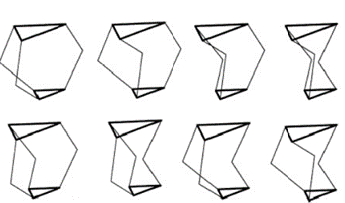
\includegraphics[width=0.5\linewidth]{delta-goalpositions.png}
    %   \caption[Die acht verschiedene Kombinationen des Vektors $\protect\vv{\theta}$ für eine eindeutige Position des Endeffektors \citefig{KaPo16}{64}.]{Die acht verschiedene Kombinationen des Vektors $\protect\vv{\theta}$ für eine eindeutige Position des Endeffektors \citefig{KaPo16}{64}.}
    %   \label{fig:delta-zielpositionen}
    % \end{figure}
    % % \newline
    % \noindent
    % Für den geometrischen Lösungsansatz wird die Topologie einer gesonderten kinematischen Kette, wie in Kapitel \ref{cap:geometrische-modellierung} beschrieben, als geschlossene Schleife betrachtet. Die Struktur beinhaltet zwei verschiedene gelenktypen, ein aktives Rotationsgelenk $A_1$ zwischen der invarianten Basis und dem proximalen Glied, welches Rotationen in der Ebene durchführen kann, sowie zwei passive Kugelgelenke $B_1$ und $C_1$, welche in der Lage sind eingeschränkt Rotationen im Raum durchzuführen. Nun können, aufgrund der spezifischen Anordnung der individuellen Gelenke und den daraus resultierenden geometrischen Eigenschaften, mathematische Zusammenhänge beschrieben werden.\\
    % \\
    % Das Rotationsgelenk $A_1$ kann nur in der von $y_0$ und $z_0$ aufgespannten Ebene rotieren und bildet folglich einen Kreis mit Mittelpunkt $A_1$ und Radius $a$. Demzufolge kann die x-Komponente des Rotationsgelenks $A_1$ vernachlässigt werden. Im Gegensatz dazu stellen die passiven Kugelgelenke $B_1$ und $C_1$ sogenannte Universalgelenke dar, dementsprechend kann sich $b$ relativ zu $C_1$ frei drehen und bildet somit eine Kugel mit Mittelpunkt $C_1$ und Radius $b$. Der Schnittpunkt dieser Kugel mit der von $y_0$ und $z_0$ aufgespannten Ebene ist ein Kreis mit Mittelpunkt $C_1'$ und Radius $\vv{C_1'B_1}$, wobei $C_1'$ die Projektion des Punktes $C_1$ auf der von $y_0$ und $z_0$ aufgespannten Ebene ist. Der Punkt $B_1$ kann als Schnittpunkt von Kreisen mit bekanntem Radius und den Mittelpunkten $C_1'$ und $A_1$ gefunden werden. Abschließend kann über den Punkt $B_1$ der Gelenkparameter $\theta\textsubscript{11}$ ermittelt werden.\\
    % \\
    % Im ersten Schritt werden die Koordinaten der Punkte $A_1$, $B_1$, $C_1$ sowie der auf die von $y_0$ und $z_0$ aufgespannte Ebene projezierte Punkt $C_1'$ im Basiskoordinatensystem ausgedrückt. Die Position des Punktes $A_1$, auf dem sich das erste aktive Rotationsgelenk befindet, wird beschrieben mit
    % \begin{align}
    %     A_1 = 
    %         \left[
    %             \begin{array}{c} 
    %                 x\textsubscript{$A1$}\\
    %                 y\textsubscript{$A1$}\\
    %                 z\textsubscript{$A1$} 
    %             \end{array}
    %         \right] =
    %         \left[
    %             \begin{array}{c} 
    %                 0\\
    %                 \frac{L \cdot tan(30)}{2}\\
    %                 0 
    %             \end{array}
    %         \right] =
    %         \left[
    %             \begin{array}{c} 
    %                 0\\
    %                 \frac{L}{2 \cdot \sqrt{3}}\\
    %                 0 
    %             \end{array}
    %         \right] =
    %         \left[
    %             \begin{array}{c} 
    %                 0\\
    %                 R\\
    %                 0 
    %             \end{array}
    %         \right]
    %     \label{eq:A1}
    % \end{align}
    % \equations{Formel \ref{eq:A1} Koordinaten des Punktes $A_1$}
    % \noindent
    % Der Punkt $B_1$, auf dem sich das erste passiv sphärische Universalgelenk befindet, sei
    % \begin{align}
    %     B_1 = 
    %         \left[
    %             \begin{array}{c} 
    %                 0\\
    %                 y\textsubscript{$B1$}\\
    %                 z\textsubscript{$B1$} 
    %             \end{array}
    %         \right]
    %     \label{eq:B1}
    % \end{align}
    % \equations{Formel \ref{eq:B1} Koordinaten des Punktes $B_1$}
    % \noindent
    % Die Position des Punktes $C_1$, auf dem sich das abschließende, passiv sphärische Universalgelenk befindet, sei
    % \begin{align}
    %     C_1 = 
    %         \left[
    %             \begin{array}{c} 
    %                 x\textsubscript{$C1$}\\
    %                 y\textsubscript{$C1$}\\
    %                 z\textsubscript{$C1$} 
    %             \end{array}
    %         \right] =
    %         \left[
    %             \begin{array}{c} 
    %                 x_p\\
    %                 y_p + \frac{l \cdot tan(30)}{2}\\
    %                 z_p 
    %             \end{array}
    %         \right] =
    %         \left[
    %             \begin{array}{c} 
    %                 x_p\\
    %                 y_p + \frac{l}{2 \cdot \sqrt{3}}\\
    %                 z_p 
    %             \end{array}
    %         \right] =
    %         \left[
    %             \begin{array}{c} 
    %                 x_p\\
    %                 y_p + r\\
    %                 z_p 
    %             \end{array}
    %         \right]
    %     \label{eq:C1}
    % \end{align}
    % \equations{Formel \ref{eq:C1} Koordinaten des Punktes $C_1$}
    % \noindent
    % Die Länge $\vv{u}$, respektive der Abstand zwischen $C_1$ und $C_1'$, wird definiert durch
    % \begin{align}
    %     \vv{u} = \vv{C_1C_1'} = \vert x_p \vert = 
    %         \left[
    %             \begin{array}{c} 
    %                 x_p\\
    %                 0\\
    %                 0 
    %             \end{array}
    %         \right]
    %     \label{eq:u}
    % \end{align}
    % \equations{Formel \ref{eq:u} Die Länge $u$, respektive der Abstand zwischen $C_1$ und $C_1'$}
    % \noindent
    % folglich kann der auf die von $y_0$ und $z_0$ aufgespannte Ebene projezierte Punkt $C_1'$ geschrieben werden als
    % \begin{align}
    %     C_1' = C_1 - \vv{u} = C_1 - \vv{C_1C_1'} =
    %         \left[
    %             \begin{array}{c} 
    %                 x\textsubscript{$C1'$}\\
    %                 y\textsubscript{$C1'$}\\
    %                 z\textsubscript{$C1'$} 
    %             \end{array}
    %         \right] =
    %         \left[
    %             \begin{array}{c} 
    %                 x\textsubscript{$C1$}\\
    %                 y\textsubscript{$C1$}\\
    %                 z\textsubscript{$C1$} 
    %             \end{array}
    %         \right] -
    %         \left[
    %             \begin{array}{c} 
    %                 x_p\\
    %                 0\\
    %                 0 
    %             \end{array}
    %         \right] =
    %         \left[
    %             \begin{array}{c} 
    %                 0\\
    %                 y_p + r\\
    %                 z_p 
    %             \end{array}
    %         \right]
    %     \label{eq:C1'}
    % \end{align}
    % \equations{Formel \ref{eq:C1'} Koordinaten des Punktes $C_1'$}
    % \noindent
    % Da bei der Berechnung der inversen Kinematik die Koordinaten des TCPs $x_p$, $y_p$ und $z_p$ als
    % gegeben betrachtet werden können, sind die Koordinaten der Punkte $A_1$, $B_1$, $C_1$ und $C_1'$ bekannt. Die Länge $\vv{v}$, respektive der z-Abstand zwischen den Punkten $C_1'$ und $B_1$, wird über den pythagoräischen Lehrsatz bestimmt
    % \begin{align}
    %     \vv{v} = \vv{C_1'B_1} = \sqrt{(\vv{C_1B_1})^2-(\vv{C_1'C_1})^2} = \sqrt{b^2 - x_p^2}
    %     \label{eq:v}
    % \end{align}
    % \equations{Formel \ref{eq:v} Die Länge $v$, respektive der z-Abstand zwischen den Punkten $C_1'$ und $B_1$}
    % \noindent
    % Anschließend wird der Vektor $\vv{w}$, respektive der Vektor zwischen den Punkten $A_1$ und $C_i'$ wie folgt ermittelt
    % \begin{align}
    %     \vv{w} = \vv{A_1C_1'} = C_1' - A_1 = 
    %         \left[
    %             \begin{array}{c} 
    %                 x_w\\
    %                 y_w\\
    %                 z_w 
    %             \end{array}
    %         \right] =
    %         \left[
    %             \begin{array}{c} 
    %                 0\\
    %                 y_p + r\\
    %                 z_p 
    %             \end{array}
    %         \right] - 
    %         \left[
    %             \begin{array}{c} 
    %                 0\\
    %                 R\\
    %                 0 
    %             \end{array}
    %         \right] = 
    %         \left[
    %             \begin{array}{c} 
    %                 0\\
    %                 y_p + r - R\\
    %                 z_p 
    %             \end{array}
    %         \right]
    %     \label{eq:w}
    % \end{align}
    % \equations{Formel \ref{eq:w} Der Vektor $w$, respektive der Vektor zwischen den Punkten $A_1$ und $C_i'$}
    % \noindent
    % Über den Konsinussatz kann der Winkel $\theta\textsubscript{21}$ ermittelt werden
    % \begin{align}
    %     cos(\theta\textsubscript{21}) = 
    %     - \frac{y_w^2 + z_w^2 - a^2 -  v^2}{2 \cdot a \cdot v}
    %     \label{eq:cos(theta21)}
    % \end{align}
    % \equations{Formel \ref{eq:cos(theta21)} Cosinus des Winkels $\theta\textsubscript{21}$}
    % \noindent
    % Unter Rücksicht des allgemeinen Ausdrucks $sin(\theta\textsubscript{21}) = \pm \sqrt{1 - cos(\theta\textsubscript{21})^2}$ kann Gleichung \ref{eq:cos(theta21)} geschrieben werden als
    % \begin{align}
    %     sin(\theta\textsubscript{21}) = 
    %     \sqrt{1 - cos(\theta\textsubscript{21})} = \sqrt{1 + \frac{y_w^2 + z_w^2 - a^2 -  v^2}{2 \cdot a \cdot v}^2}
    %     \label{eq:sin(theta21)}
    % \end{align}
    % \equations{Formel \ref{eq:sin(theta21)} Sinus des Winkels $\theta\textsubscript{21}$}
    % \noindent
    % Nun kann $\theta\textsubscript{21}$ mit dem  \textit{erweiterten Arcustangens} berechnet werden
    % \begin{align}
    %     \theta\textsubscript{21} = arctan2( sin(\theta\textsubscript{21}), cos(\theta\textsubscript{21}) ) = arctan2\left( \sqrt{1 + \frac{y_w^2 + z_w^2 - a^2 -  v^2}{2 \cdot a \cdot v}^2}, \pm \frac{y_w^2 + z_w^2 - a^2 -  v^2}{2 \cdot a \cdot v} \right)
    %     \label{eq:theta21}
    % \end{align}
    % \equations{Formel \ref{eq:theta21} Winkel $\theta\textsubscript{21}$}
    % \noindent
    % Unter Zuhilfenahme des berechneten Winkels $\theta\textsubscript{21}$ ist es nun möglich, den Winkel des ersten distalen Gliedes $\theta\textsubscript{11}$, respektive die Winkelstellung des ersten Aktors, zu berechnen.
    % \begin{align}
    %     \theta\textsubscript{11} = 
    %     atan2(y_w, z_w) - atan2(v \cdot sin(\theta\textsubscript{21}), a + v \cdot cos(\theta\textsubscript{21})))
    %     \label{eq:theta11}
    % \end{align}
    % \equations{Formel \ref{eq:theta11} Winkel des ersten distalen Gliedes $\theta\textsubscript{11}$}
    % \noindent
    
    
    % \newpage
    \section{Inverse Kinematik} % Hieger
    
    Bei der inversen Kinematik ist die Pose des Endeffektors, respektive die Lage des Arbeitspunktes am Ende der kinematischen Kette, der sogenannte TCP (von engl. Tool Center Point), gegeben. Wie im vorigen Abschnitt \ref{sec:DoF} beschrieben, fungiert der Delta-Roboter als kartesische Positioniereinrichtung mit drei Freiheitsgraden in x, y und z-Richtung, welche durch die drei Koordinaten $x_p$, $y_p$ und $z_p$, im Basiskoordinatensystem ausgedrückt, beschrieben werden.\\
    \\
    Die Berechnung des Vektors $\vv{\theta}$, bestehend aus den aktiven Gelenkvariablen, liefert multiple Lösungen. Dies kann zu Problemen führen, da das System eine davon auswählen muss. Es existieren jedoch bereits verschiedene Ansätze mit diversen Kriterien um die Entscheidung zu beeinflussen und eine eindeutige Lösung zu erhalten. Eine etablierte Herangehensweise ist die Wahl der nächstliegenden Lösung, respektive jener, bei der sich die Gelenke des Endeffektors möglichst wenig bewegen. Jede kinematische Kette des Delta-Roboters kann gesondert betrachtet eine beliebige Position auf zwei verschiedene Lösungsarten erreichen, die drei kinematischen Ketten zu einem geschlossenen System zusammengefasst ergeben jedoch sogar acht verschiedene Kombinationen des Vektors $\vv{\theta}$, um eine eindeutige Position des Endeffektors zu erreichen, veranschaulicht in Abbildung \ref{fig:delta-zielpositionen} \cite{KaPo16}.
    \begin{figure}[H]
      \centering
      %\fbox
      {
        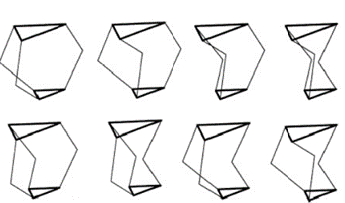
\includegraphics[width=0.5\linewidth]{delta-goalpositions.png}
      }
      \caption[Die acht verschiedene Kombinationen des Vektors $\protect\vv{\theta}$ für eine eindeutige Position des Endeffektors \citefig{KaPo16}{64}]{Die acht verschiedene Kombinationen des Vektors $\protect\vv{\theta}$ für eine eindeutige Position des Endeffektors \citefig{KaPo16}{64}}
      \label{fig:delta-zielpositionen}
    \end{figure}
    % \newline
    \noindent
    Für den geometrischen Lösungsansatz wird die Topologie einer gesonderten kinematischen Kette, wie in Kapitel \ref{cap:geometrische-modellierung} beschrieben, als geschlossene Schleife betrachtet. Die Struktur beinhaltet zwei verschiedene Gelenktypen, ein aktives Rotationsgelenk $F_1$ zwischen der invarianten Basis und dem proximalen Glied, welches Rotationen in der Ebene durchführen kann, sowie zwei passive Kugelgelenke $J_1$ und $E_1$, welche in der Lage sind eingeschränkt Rotationen im Raum durchzuführen. Nun können, aufgrund der spezifischen Anordnung der individuellen Gelenke und den daraus resultierenden geometrischen Eigenschaften, mathematische Zusammenhänge beschrieben werden. Der Gelenkparameter $\theta\textsubscript{11}$ kann über den Anbindungspunkt $J_1$ ermittelt werden, welcher wiederum als Schnittpunkt zweier Kreise, wie in der folgenden Abbildung \ref{fig:delta-param-isometric-view} dargestellt, beschrieben werden kann.
    \begin{figure}[H] 
      \centering
      %\fbox
      {
        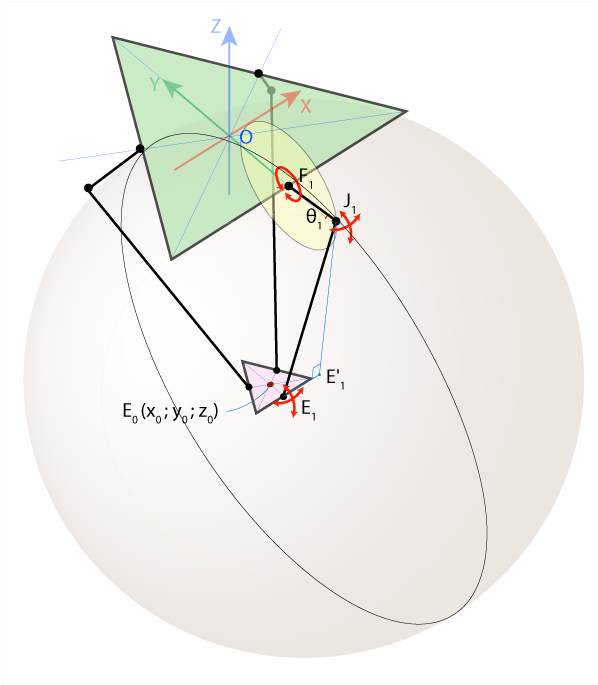
\includegraphics[width=0.5\linewidth]{delta-param-isometric-view.png}
      }
      \caption[Bewegungsparameter der Robotergelenke \citefig{PoUr11}{437}]{Bewegungsparameter der Robotergelenke \citefig{PoUr11}{437}}
      \label{fig:delta-param-isometric-view}
    \end{figure}
    % \newline
    \noindent
    Im ersten Schritt werden die Koordinaten der Punkte $F_1$, $J_1$, $E_1$ sowie der auf die von $y_0$ und $z_0$ aufgespannte Ebene projezierte Punkt $E_1'$ im Basiskoordinatensystem ausgedrückt. Die Position des Punktes $F_1$, auf dem sich das erste aktive Rotationsgelenk befindet, wird beschrieben mit
    \newline
    \begin{align}
        F_1 = 
            \left[
                \begin{array}{c} 
                    x\textsubscript{$F1$}\\
                    y\textsubscript{$F1$}\\
                    z\textsubscript{$F1$} 
                \end{array}
            \right] =
            \left[
                \begin{array}{c} 
                    0\\
                    - \frac{L \cdot tan(30)}{2}\\
                    0 
                \end{array}
            \right] =
            \left[
                \begin{array}{c} 
                    0\\
                    - \frac{L}{2 \cdot \sqrt{3}}\\
                    0 
                \end{array}
            \right] =
            \left[
                \begin{array}{c} 
                    0\\
                    - R\\
                    0 
                \end{array}
            \right]
        \label{eq:F1}
    \end{align}
    \equations{Formel \ref{eq:F1} Koordinaten des Punktes $F_1$}
    \noindent
    Der Punkt $J_1$, auf dem sich das erste passiv sphärische Universalgelenk befindet, sei
    \newline
    \begin{align}
        J_1 = 
            \left[
                \begin{array}{c} 
                    0\\
                    y\textsubscript{$J1$}\\
                    z\textsubscript{$J1$} 
                \end{array}
            \right]
        \label{eq:J1}
    \end{align}
    \equations{Formel \ref{eq:J1} Koordinaten des Punktes $J_1$}
    \noindent
    Die Position des Punktes $E_1$, auf dem sich das abschließende, passiv sphärische Universalgelenk befindet, sei
    \newline
    \begin{align}
        E_1 = 
            \left[
                \begin{array}{c} 
                    x\textsubscript{$E1$}\\
                    y\textsubscript{$E1$}\\
                    z\textsubscript{$E1$} 
                \end{array}
            \right] =
            \left[
                \begin{array}{c} 
                    x_p\\
                    y_p - \frac{l \cdot tan(30)}{2}\\
                    z_p 
                \end{array}
            \right] =
            \left[
                \begin{array}{c} 
                    x_p\\
                    y_p - \frac{l}{2 \cdot \sqrt{3}}\\
                    z_p 
                \end{array}
            \right] =
            \left[
                \begin{array}{c} 
                    x_p\\
                    y_p - r\\
                    z_p 
                \end{array}
            \right]
        \label{eq:E1}
    \end{align}
    \equations{Formel \ref{eq:E1} Koordinaten des Punktes $E_1$}
    \noindent
    Die Länge $\vv{u}$, respektive der Abstand zwischen $E_1$ und $E_1'$, wird definiert durch
    \newline
    \begin{align}
        \vv{u} = \vv{E_1E_1'} = \vert x_p \vert = 
            \left[
                \begin{array}{c} 
                    x_p\\
                    0\\
                    0 
                \end{array}
            \right]
        \label{eq:u}
    \end{align}
    \equations{Formel \ref{eq:u} Die Länge $u$, respektive der Abstand zwischen $E_1$ und $E_1'$}
    \noindent
    folglich kann der auf die von $y_0$ und $z_0$ aufgespannte Ebene projezierte Punkt $E_1'$ geschrieben werden als
    \newline
    \begin{align}
        E_1' = E_1 - \vv{u} = E_1 - \vv{E_1E_1'} =
            \left[
                \begin{array}{c} 
                    x\textsubscript{$E1'$}\\
                    y\textsubscript{$E1'$}\\
                    z\textsubscript{$E1'$} 
                \end{array}
            \right] =
            \left[
                \begin{array}{c} 
                    x\textsubscript{$E1$}\\
                    y\textsubscript{$E1$}\\
                    z\textsubscript{$E1$} 
                \end{array}
            \right] -
            \left[
                \begin{array}{c} 
                    x_p\\
                    0\\
                    0 
                \end{array}
            \right] =
            \left[
                \begin{array}{c} 
                    0\\
                    y_p - r\\
                    z_p 
                \end{array}
            \right]
        \label{eq:E1'}
    \end{align}
    \equations{Formel \ref{eq:E1'} Koordinaten des Punktes $E_1'$}
    \noindent
    Da bei der Berechnung der inversen Kinematik die Koordinaten des TCPs $x_p$, $y_p$ und $z_p$ als
    gegeben betrachtet werden können, sind die Koordinaten der Punkte $F_1$, $J_1$, $E_1$ und $E_1'$ bekannt. Um die beiden Unbekannten des Punktes $J_1$, $y\textsubscript{$J1$}$ und $z\textsubscript{$J1$}$, zu ermitteln, wird zuerst die Länge $\vv{v}$, respektive der z-Abstand zwischen $E_1'$ und $J_1$ über den pythagoräischen Lehrsatz bestimmt
    \newline
    \begin{align}
        \vv{v} = \vv{E_1'J_1} = \sqrt{(\vv{E_1J_1})^2-(\vv{E_1'E_1})^2} = \sqrt{b^2 - x_p^2} \Rightarrow v^2 = b^2 - x_p^2
        \label{eq:v}
    \end{align}
    \equations{Formel \ref{eq:v} Die Länge $v$, respektive der z-Abstand zwischen $E_1'$ und $J_1$}
    \noindent
    Das Rotationsgelenk $F_1$ kann nur in der von $y_0$ und $z_0$ aufgespannten Ebene rotieren und bildet folglich einen Kreis $K$ mit Mittelpunkt $F_1$ und Radius $a$. Demzufolge kann die x-Komponente des Rotationsgelenks $F_1$ vernachlässigt werden. Im Gegensatz dazu stellen die passiven Kugelgelenke $J_1$ und $E_1$ sogenannte Universalgelenke dar, dementsprechend kann sich $b$ relativ zu $E_1$ frei drehen und bildet somit eine Kugel mit Mittelpunkt $E_1$ und Radius $b$. Der Schnittpunkt dieser Kugel mit der von $y_0$ und $z_0$ aufgespannten Ebene ist ein Kreis $k$ mit Mittelpunkt $E_1'$ und Radius $\vv{v}$, wobei $E_1'$ die Projektion des Punktes $E_1$ auf der von $y_0$ und $z_0$ aufgespannten Ebene ist. Wie in Abbildung \ref{fig:delta-param-side-view} ersichtlich kann der Punkt $J_1$ als Schnittpunkt der beiden Kreise $K$ und $k$, da sowohl die Radii $a$ und $v$ als auch die Mittelpunkte $E_1'$ und $F_1$ bekannt sind, gefunden werden.
    \begin{figure}[H] 
      \centering
      %\fbox
      {
        \includegraphics[width=0.5\linewidth]{delta-param-side-view.tikz}
      }
      \caption[Projektion des Roboters auf die von von $y_0$ und $z_0$ aufgespannte Ebene zur Ermittlung des Schnittpunkt $J_1$]{Projektion des Roboters auf die von von $y_0$ und $z_0$ aufgespannte Ebene zur Ermittlung des Schnittpunkt $J_1$}
      \label{fig:delta-param-side-view}
    \end{figure}
    % \newline
    \noindent
    Unter Rücksicht der allgemeinen Kreisgleichung mit Mittelpunkt $(m_1, m_2)$ und Radius $r$  
    \newline
    \begin{align}
        r^2 = (x - m_1)^2 + (y - m_2)^2
        \label{eq:kreisgleichung_allgemein}
    \end{align}
    \equations{Formel \ref{eq:kreisgleichung_allgemein} Kreisgleichung}
    \noindent
    sei die Kreisgleichung des ersten Kreises $K$ 
    \newline
    \begin{align}
        a^2 = (y\textsubscript{$J1$} - y\textsubscript{$F1$})^2 + (z\textsubscript{$J1$} - z\textsubscript{$F1$})^2 = (y\textsubscript{$J1$} + R)^2 + z\textsubscript{$J1$}^2
        \label{eq:kreisgleichung_K}
    \end{align}
    \equations{Formel \ref{eq:kreisgleichung_K} Kreisgleichung des Kreises $K$}
    \noindent
    und die des zweiten Kreises $k$ 
    \newline
    \begin{align}
        v^2 = (y\textsubscript{$J1$} - y\textsubscript{$E1'$})^2 + (z\textsubscript{$J1$} - z\textsubscript{$E1'$})^2 = (y\textsubscript{$J1$} - y_0 + r)^2 + (z\textsubscript{$J1$} - z_p)^2
        \label{eq:kreisgleichung_k}
    \end{align}
    \equations{Formel \ref{eq:kreisgleichung_k} Kreisgleichung des Kreises $k$}
    \noindent
    Um nun den Schnittpunkt $J_1$ zu erhalten wird aus den Gleichungen \ref{eq:kreisgleichung_K} und \ref{eq:kreisgleichung_k} ein Gleichungssystem mit den beiden Unbekannten $y\textsubscript{$J1$}$ und $z\textsubscript{$J1$}$ aufgestellt.
    \newline
    \begin{align}
        J_1 = 
            \left[
                \begin{array}{c} 
                    y\textsubscript{$J1$}\\
                    z\textsubscript{$J1$} 
                \end{array}
            \right] =
            \begin{cases}
                a^2 = (y\textsubscript{$J1$} + R)^2 + z\textsubscript{$J1$}^2\\
                v^2 = (y\textsubscript{$J1$} - y_0 + r)^2 + (z\textsubscript{$J1$} - z_p)^2
            \end{cases}
        \label{eq:J1-gleichungssystem}
    \end{align}
    \equations{Formel \ref{eq:J1-gleichungssystem} Gleichungssystems zur Ermittlung des Anbindungspunktes $J_1$}
    \noindent
    Gleichung \ref{eq:kreisgleichung_K} kann wie folgt umgeformt werden
    \newline
    \begin{align}
        z\textsubscript{$J1$}^2 = a^2 - (y\textsubscript{$J1$} - y\textsubscript{$F1$})^2 + (z\textsubscript{$J1$} - z\textsubscript{$F1$})^2 = (y\textsubscript{$J1$} + R)^2 
        \label{eq:kreisgleichung_K-umgeformt}
    \end{align}
    \equations{Formel \ref{eq:kreisgleichung_K-umgeformt} Umgeformte Kreisgleichung des Kreises $K$}
    \noindent
    wird nun $z\textsubscript{$J1$}$ in Gleichung \ref{eq:kreisgleichung_k} mit dem aus Gleichung \ref{eq:kreisgleichung_K-umgeformt} erhaltenen Ausdruck ersetzt erhält man eine Lösung in der Form
    \newline
    \begin{align}
        z\textsubscript{$J1$} = e + f \cdot y\textsubscript{$J1$}
        \label{eq:zJ1}
    \end{align}
    \equations{Formel \ref{eq:zJ1} Umgeformte Kreisgleichung des Kreises $K$}
    \noindent
    wobei die beiden Hilfsvariablen $e$ und $f$ definiert sind als
    \newline
    \begin{align}
        e = \frac{x_p^2 + (y_p - r)^2 + z_p^2 + a^2 - b^2 + R^2}{2 \cdot z_p} \nonumber \\
        f = \frac{r-R-y_p}{z_p}
        \label{eq:ef}
    \end{align}
    \equations{Formel \ref{eq:ef} Helfervariablen}
    \noindent
    Die Berechnung für $y\textsubscript{$J1$}$ liefert eine quadratische Gleichung und somit zwei Lösungen, in Abbildung \ref{fig:delta-param-side-view} durch die zwei Schnittpunkte der Kreise dargestellt. Aufgrund der Orientierung des Arms ist jedoch nur die größere der beiden Lösungen zweckmäßig und somit ausschlaggebend. Die kleinere Lösung, welche den inneren Schnittpunkt der beiden Kreise repräsentiert, kann somit vernachlässigt werden.
    % \begin{align}
    %     y\textsubscript{$J1$} = \frac{-R - e \cdot f - \sqrt{D}}{f^2 + 1}\\
    %     \label{eq:yJ1zJ1}
    % \end{align}
    % \equations{Formel \ref{eq:yJ1zJ1} Gelenkparameter}
    % \noindent
    % $D$ sei die Diskriminante der quadratischen Gleichung, respektive jener Rechenausdruck welcher Aussagen über Zahl und Art der Lösungen einer algebraischen Gleichung ermöglicht
    % \begin{align}
    %     D = -(e + f \cdot (-R))^2 + a^2 \cdot (f^2 + 1)
    %     \label{eq:D}
    % \end{align}
    % \equations{Formel \ref{eq:D} Diskriminante der quadratischen Gleichung}
    % \noindent
    Unter Zuhilfenahme des zuvor berechneten Anbindungspunktes $J_1$ ist es nun möglich, den Winkel des ersten distalen Gliedes $\theta\textsubscript{11}$, respektive die Winkelstellung des ersten Aktors, zu berechnen.
    \newline
    \begin{align}
        \theta\textsubscript{11} = arctan\left(\frac{z\textsubscript{$J1$}}{y\textsubscript{$F1$} - y\textsubscript{$J1$}}\right)
        \label{eq:theta11}
    \end{align}
    \equations{Formel \ref{eq:theta11} Winkel des ersten distalen Gliedes $\theta\textsubscript{11}$}
    \noindent
    Unbekannte Gelenkwinkel dürfen nicht über den Arcussinus oder Arcuskosinus berechnet werden, da der Arcussinus nur Werte im Intervall $[\frac{-\pi}{2}, \frac{\pi}{2}]$ und der Arcuskosinus nur Werte im Intervall $[0, \pi]$ liefert. Zudem ist der Definitionsbereich der beiden Arcusfunktionen auf das Intervall $[-1, 1]$ beschränkt. Gleichwohl liefert auch der Arcustangens nur Werte im Intervall $(\frac{-\pi}{2}, \frac{\pi}{2})$, da die Tangensfunktion für Funktionswerte von $\pm \frac{\pi}{2}$ nicht umkehrbar ist. Um Lösungsverluste zu vermeiden und beliebige Positionen des Endeffektors erreichen zu können ist es unabdingbar, unbekannte Gelenkwinkel der Gleichungssysteme über den \textit{erweiterten Arcustangens} zu berechnen. Der Funktion werden zwei Argumente übergeben, wobei das zweite Argument gleich dem Nenner ist, welcher jedoch Null sein darf, da durch Auswertung der Vorzeichen der beiden Argumente der Quadrant des Ergebnisses bestimmt wird. Somit liefert der \textit{erweiterte Arcustangens} Werte im Intervall $(-\pi, \pi]$. Sollten beide Argumente der Funktion Null sein, so ist diese mathematisch nicht definiert und die erhaltene Konfiguration des Endeffektors demnach unzulässig \cite{We08}.\\
    \\
    Durch den rotationssymmetrischen Aufbau des Delta-Roboters ist eine vereinfachte Bestimmung der Winkel $\theta\textsubscript{12}$ und $\theta\textsubscript{13}$ der beiden anderen distalen Glieder, respektive die Winkelstellungen der weiteren Aktoren, möglich. Um hierbei aus dem globalen Basiskoordinatensystem $O$ in die lokalen, gliederseitigen Koordinatensysteme $F_i$ zu gelangen, können die Abzisse $x_0$ und Ordinate $y_0$ nach der in Kapitel \ref{cap:geometrische-modellierung} eingeführten Rotationsmatrix  mit 120 beziehungsweise 240 $[^{\circ}]$ um die Applikate $z_0$ gegen den Uhrzeigersinn gedreht werden. Zudem werden die gegebenen Koordinaten des TCPs $x_p$, $y_p$ und $z_p$ mit Hilfe der Rotationsmatrix im entsprechenden Koordinatensystem abgebildet. Mit den transformierten Koordinaten kann nun eine wiederholte Berechnung des jeweiligen Winkels auf Basis der Gleichungen \ref{eq:F1} bis \ref{eq:theta11} erfolgen. Die Transformation liefert für das Gelenk $F_2$ die Koordinaten
    \newline
    \begin{align}
        F_2 =
            \left[
                \begin{array}{c} 
                    x\textsubscript{$F2$}\\
                    y\textsubscript{$F2$}\\
                    z\textsubscript{$F2$} 
                \end{array}
            \right] =
            \left[
                \begin{array}{c} 
                    x_0 \cdot cos(120) + y_0 \cdot sin(120)\\
                    - x_0 \cdot cos(120) + y_0 \cdot sin(120)\\
                    z_0 
                \end{array}
            \right]
        \label{eq:F2}
    \end{align}
    \equations{Formel \ref{eq:F2} Koordinaten des Punktes $F_2$}
    \noindent
    und für das Gelenk $F_3$ die Koordinaten
    \begin{align}
        F_3 =
            \left[
                \begin{array}{c} 
                    x\textsubscript{$F3$}\\
                    y\textsubscript{$F3$}\\
                    z\textsubscript{$F3$} 
                \end{array}
            \right] =
            \left[
                \begin{array}{c} 
                    x_0 \cdot cos(240) + y_0 \cdot sin(240)\\
                    - x_0 \cdot cos(240) + y_0 \cdot sin(240)\\
                    z_0 
                \end{array}
            \right]
        \label{eq:F3}
    \end{align}
    \equations{Formel \ref{eq:F3} Koordinaten des Punktes $F_3$}
    \noindent
    
    
    % \newpage
    % \section{Inverse Kinematik} % Bouzgou

    % Für den geometrischen Lösungsansatz wird die Topologie einer gesonderten kinematischen Kette als geschlossene Schleife betrachtet. Daraus resultierend kann die Kette $OA_iB_iC_iP$ mit folgender Schleifenschlussgleichung eines isolierten Gliedmaßes $i$ gebildet werden: 
    % \begin{align}
    %     \vv{OP} + \vv{PC_i} = \vv{OA_i} + \vv{A_iB_i} + \vv{B_iC_i} \equiv \vv{p} + \vv{r} = \vv{R} + \vv{a} + \vv{b} \Rightarrow \vv{p} = \vv{R} + \vv{a} + \vv{b} - \vv{r}
    %     \label{eq:schleifenschlussgleichung}
    % \end{align}
    % \equations{Formel \ref{eq:schleifenschlussgleichung} Schleifenschlussgleichung}
    % In Matrixschreibweise geschrieben als
    % \begin{align}
    %     \left[
    %         \begin{array}{c} 
    %             x_p \cdot cos(\alpha) - y_p \cdot sin(\alpha)\\
    %             x_p \cdot sin(\alpha) + y_p \cdot cos(\alpha)\\
    %             z_p
    %         \end{array}
    %     \right]  =
    %     \left[
    %         \begin{array}{c} 
    %             R\\
    %             0\\
    %             0
    %         \end{array}
    %     \right] + a 
    %     \left[
    %         \begin{array}{c} 
    %             cos(\theta\textsubscript{1i})\\
    %             0\\
    %             sin(\theta\textsubscript{1i})
    %         \end{array}
    %     \right] + b 
    %     \left[
    %         \begin{array}{c} 
    %             sin(\theta\textsubscript{3i}) \cdot cos(\theta\textsubscript{2i} + \theta\textsubscript{1i})\\
    %             cos(\theta\textsubscript{3i})\\
    %             sin(\theta\textsubscript{3i}) \cdot
    %             sin(\theta\textsubscript{2i} + \theta\textsubscript{1i})
    %         \end{array}
    %     \right] - 
    %     \left[
    %         \begin{array}{c} 
    %             r\\
    %             0\\
    %             0
    %         \end{array}
    %     \right]
    %     \label{eq:schleifenschlussgleichung-matrixschreibweise}
    % \end{align}
    % \equations{Formel \ref{eq:schleifenschlussgleichung-matrixschreibweise} Schleifenschlussgleichung (matrixschreibweise)}
    % Den Winkel $\theta\textsubscript{3i}$ erhält man durch Umformen des zweiten Zeilenvektors der Gleichung \ref{eq:schleifenschlussgleichung-matrixschreibweise}. 
    % \begin{align}
    %     \theta\textsubscript{3i} = 
    %         cos\textsuperscript{-1}(\frac{1}{b} \cdot (x_p \cdot sin(\alpha) + y_p \cdot cos(\alpha))
    %     \label{eq:zweiter-zeilenvektor}
    % \end{align}
    % \equations{Formel \ref{eq:zweiter-zeilenvektor} Zweiter Zeilenvektor der Schleifenschlussgleichung}
    % Nun erhält man ein Gleichungssystem mit zwei unbekannten Variablen welches gelöst werden kann indem zunächst der erste und dritte Zeilenvektor gleich Null gesetzt werden
    % \begin{align}
    %     x_p \cdot cos(\alpha) - y_p \cdot sin(\alpha) - R - a \cdot cos(\theta\textsubscript{1i}) - b \cdot sin(\theta\textsubscript{3i}) \cdot cos(\theta\textsubscript{2i} + \theta\textsubscript{1i}) + r = 0
    %     \label{eq:erster-zeilenvektor}\\
    %     z_p - a \cdot sin(\theta\textsubscript{1i}) - b \cdot sin(\theta\textsubscript{3i}) \cdot sin(\theta\textsubscript{2i} + \theta\textsubscript{1i}) = 0
    %     \label{eq:dritter-zeilenvektor}
    % \end{align}
    % \equations{Formel \ref{eq:erster-zeilenvektor} Erster Zeilenvektor der Schleifenschlussgleichung}
    % \equations{Formel \ref{eq:dritter-zeilenvektor} Dritter Zeilenvektor der Schleifenschlussgleichung}
    % Werden nun Gleichung \ref{eq:erster-zeilenvektor} und \ref{eq:dritter-zeilenvektor} gleichgesetzt folgt
    % \begin{align*}
    %     (x_p \cdot cos(\alpha) - y_p \cdot sin(\alpha) - R - a \cdot cos(\theta\textsubscript{1i}) - b \cdot sin(\theta\textsubscript{3i}) \cdot cos(\theta\textsubscript{2i} + \theta\textsubscript{1i}) + r)^2 =\\ 
    %     (z_p - a \cdot sin(\theta\textsubscript{1i}) - b \cdot sin(\theta\textsubscript{3i}) \cdot sin(\theta\textsubscript{2i} + \theta\textsubscript{1i}))^2
    %     % \label{eq:zeilenvektoren-gleichgesetzt}
    % \end{align*}
    % % \equations{Formel \ref{eq:zeilenvektoren-gleichgesetzt} Zeilenvektoren (gleichgesetzt)}
    % Dies kann in vereinfachter Form geschrieben werden als
    % \begin{align}
    %     (x_p \cdot cos(\alpha) - y_p \cdot sin(\alpha) - R - a \cdot cos(\theta\textsubscript{1i}) + r)^2 = 
    %     (b \cdot sin(\theta\textsubscript{3i}))^2 \textbf{- (?)} z_p - a \cdot sin(\theta\textsubscript{1i})
    %     \label{eq:zeilenvektoren-vereinfacht}
    % \end{align}
    % \equations{Formel \ref{eq:zeilenvektoren-vereinfacht} Zeilenvektoren (vereinfacht)}
    % und anschließend umgeformt werden auf
    % \begin{align}
    %     (b \cdot sin(\theta\textsubscript{3i}))^2 =
    %     (x_p \cdot cos(\alpha) - y_p \cdot sin(\alpha) - R - a \cdot cos(\theta\textsubscript{1i}) + r + z_p + a \cdot sin(\theta\textsubscript{1i}))^2
    %     \label{eq:zeilenvektoren-umgeformt}
    % \end{align}
    % \equations{Formel \ref{eq:zeilenvektoren-umgeformt} Zeilenvektoren (umgeformt)}
    % Unter Rücksicht des allgemeinen Ausdrucks $sin(cos\textsuperscript{-1}(x)) = \sqrt{1-x^2}$ kann Gleichung \ref{eq:zweiter-zeilenvektor} geschrieben werden als
    % \begin{align*}
    %     \theta\textsubscript{3i} = 
    %         cos\textsuperscript{-1}(\frac{1}{b} \cdot (x_p \cdot sin(\alpha) + y_p \cdot cos(\alpha))) \Rightarrow\\
    %     b \cdot sin(\theta\textsubscript{3i}) = 
    %         b \cdot \sqrt{1 - (\frac{1}{b} \cdot (x_p \cdot sin(\alpha) + y_p \cdot cos(\alpha)))^2} \Rightarrow\\
    %     (b \cdot sin(\theta\textsubscript{3i}))^2 = 
    %         b^2 - (x_p \cdot sin(\alpha) + y_p \cdot cos(\alpha))^2
    %     % \label{eq:zweiter-zeilenvektor-umgeformt}
    % \end{align*}
    % % \equations{Formel \ref{eq:zweiter-zeilenvektor-umgeformt} Zweiter Zeilenvektoren (umgeformt)}
    % Daraus folgt
    % \begin{align*}
    %     b^2 - (x_p \cdot sin(\alpha) + y_p \cdot cos(\alpha))^2 = (x_p \cdot cos(\alpha) - y_p \cdot sin(\alpha) - R + r + z_p + a \cdot (sin(\theta\textsubscript{1i}) - cos(\theta\textsubscript{1i})))^2
    %     % \label{eq:zweiter-zeilenvektor-vereinfacht}
    % \end{align*}
    % % \equations{Formel \ref{eq:zweiter-zeilenvektor-vereinfacht} Zweiter Zeilenvektoren (vereinfacht)}
    % in weiterer Folge kann die Gleichung aufgeteilt werden in
    % \begin{align*}
    %     A = b^2 - (x_p \cdot sin(\alpha) + y_p \cdot cos(\alpha))^2\\
    %     B = x_p \cdot cos(\alpha) - y_p \cdot sin(\alpha) - R + r + z_p 
    % \end{align*}
    % Nun kann Gleichung \ref{eq:zeilenvektoren-vereinfacht} in folgender Form geschrieben werden:
    % \begin{align*}
    %     A^\frac{1}{2} = B + a \cdot (sin(\theta\textsubscript{1i}) - cos(\theta\textsubscript{1i})) \Rightarrow\\
    %     sin(\theta\textsubscript{1i}) = \frac{1}{a} \cdot (A^\frac{1}{2} - B) + cos(\theta\textsubscript{1i})
    % \end{align*}
    % Wird die Gleichung auf $\theta\textsubscript{1i}$ umgeformt resultiert dies in zwei Lösungen des Gelenkwinkels
    % \begin{align*}
    %     \theta\textsubscript{1i} = cos\textsuperscript{-1}\left(\frac{1}{2} \cdot \left(\frac{A^\frac{1}{2} - B}{a}\right) \pm \left(\left(\frac{A^\frac{1}{2} - B}{a}\right)^2 - 2\right)\right)
    % \end{align*}
    
    
    %%%%%%%%%%%%%%%%%%%%%%%%%%%%%%%%%%%%%%%%%%%%%%%%%%%%%%%%%%%%%%%%%%%%%%%%%%%%%%%%%%%%%%%%%%%%%%%%%%%%%%%%
    
    % vereinfacht zu
    % \begin{align*}
    %     (a \cdot (sin(\theta\textsubscript{1i}) - cos(\theta\textsubscript{1i})))^2 = b^2 - (x_p \cdot sin(\alpha) + y_p \cdot cos(\alpha))^2 - (x_p \cdot cos(\alpha) - y_p \cdot sin(\alpha) - R + r + z_p)^2
    % \end{align*}
    % in weiterer Folge
    % \begin{align}
    %     sin(\theta\textsubscript{1i}) - cos(\theta\textsubscript{1i}) = \frac{1}{a} \cdot (b - (x_p \cdot sin(\alpha) + y_p \cdot cos(\alpha)) - (x_p \cdot cos(\alpha) - y_p \cdot sin(\alpha) - R + r + z_p))
    %     \label{eq:theta1i}
    % \end{align}
    % Unter Rücksicht des allgemeinen Ausdrucks $sin^-1(cos(x)) = x + \frac{\pi}{2}$ kann Gleichung \ref{eq:theta1i} geschrieben werden als
    % \begin{align*}
    %     \theta\textsubscript{1i} - cos(\theta\textsubscript{1i}) = \frac{1}{a} \cdot (b - (x_p \cdot sin(\alpha) + y_p \cdot cos(\alpha)) - (x_p \cdot cos(\alpha) - y_p \cdot sin(\alpha) - R + r + z_p))
    %     % \label{eq:theta1i}
    % \end{align*}
    

    %%%%%%%%%%%%%%%%%%%%%%%%%%%%%%%%%%%%%%%%%%%%%%%%%%%%
    %%                 Jacobi-Matrix                  %%
    %%%%%%%%%%%%%%%%%%%%%%%%%%%%%%%%%%%%%%%%%%%%%%%%%%%%
    % \newpage
    \section{Jacobi-Matrix}
    \label{cap:jacobi}
    
    Um die inverse Kinematik für jeden beliebigen Robotertyp analytisch zu bestimmen muss auf näherungsweise Berechnungsverfahren, etwa auf Basis der \textit{Jacobi–Matrix}, zurückgegriffen werden. Diese, nach dem Mathematiker \textit{Carl Gustav Jacob Jacobi} (1804 – 1851) benannte Ableitungsmatrix, beschreibt den Zusammenhang zwischen den Gelenkgeschwindigkeiten und der Geschwindigkeit des Endeffektors im kartesischen Raum durch eine Matrix mit der Dimension $6 \times n$, wobei $n$ die Anzahl der Gelenkachsen des Roboters ist, das heißt jede Spalte entspricht einer Gelenkachse \cite{We08}.\\
    \\
    Die größten Herausforderungen bei der Berechnung der \textit{Jacobi–Matrix} paralleler Roboter liegen in der geschlossenen kinematischen Struktur, da nicht jeder Antrieb unabhängig betrieben werden kann und die Struktur passive Gelenke enthält, welche in der Berechnung berücksichtigt werden müssen.\\
    \\
    Die Notation der \textit{Jacobi-Matrix} des Delta-Roboters können den beiden folgenden Abbildungen \ref{fig:top-view-jacobi} und \ref{fig:delta-closed-loop-jacobi} mit Drauf- und Seitenansicht des Delta-Roboters entnommen werden.
    \begin{figure}[H]
        \centering
        %\fbox
        {
            \includegraphics[width=0.85\linewidth]{top-view.tikz}
        }
        \caption[Draufsicht mit Notation der invarianten Basis (links) und beweglichen Plattform (rechts) des Delta-Roboters]{Draufsicht mit Notation der invarianten Basis (links) und beweglichen Plattform (rechts) des Delta-Roboters}
        %\citefigm{Wi16}
        \label{fig:top-view-jacobi}
    \end{figure}
    % \newline
    \noindent
    \begin{figure}[H]
        \centering
        %\fbox
        {
            \includegraphics[width=0.85\linewidth]{delta-closed-loop.tikz}
        }
        \caption[{Seitenansicht mit Notation der Kinematik einer geschlossenen Kette des Delta-Roboters (links), analoge Kette, -90 $[^{\circ}]$ um $z_o$ gedreht (rechts)}]{Seitenansicht mit Notation der Kinematik einer geschlossenen Kette des Delta-Roboters (links), analoge Kette, -90 $[^{\circ}]$ um $z_o$ gedreht (rechts)}
        % \citefigm{LyPa17}
        \label{fig:delta-closed-loop-jacobi}
    \end{figure}
    % \newline
    \noindent
    Um die \textit{Jacobi–Matrix} eines Delta-Roboters zu bestimmen, sollte im ersten Schritt die relevanteste kinematische Kette des Roboters, analog der Vorgehensweise aus Kapitel \ref{cap:mathematische-modellierung}, herangezogen werden. Anschließend wird die \textit{Jacobi–Matrix} durch Differenzieren der geeigneten Schleifenschlussgleichung und Neuanordnung des Ergebnisses in folgender Form abgeleitet
    \newline
    \begin{align}
        \vv{J}_\theta = 
            \left[
                \begin{array}{c} 
                    \dot{\theta\textsubscript{11}}\\
                    \dot{\theta\textsubscript{12}}\\
                    \dot{\theta\textsubscript{13}} 
                \end{array}
            \right]
        = \vv{J}_p = 
            \left[
                \begin{array}{c} 
                    \dot{x_p} = v_x\\
                    \dot{y_p} = v_y\\
                    \dot{z_p} = v_z 
                \end{array}
            \right]
        \label{eq:jacobi}
    \end{align}
    \equations{Formel \ref{eq:jacobi} Jacobi-Matrix}
    \noindent
    Dabei sind $v_x$, $v_y$ und $v_z$ die x-, y- und z-Komponenten der Geschwindigkeit des Punktes P auf der beweglichen Plattform im Intertialkoordinatensystem $O$.\\
    \\
    Um die in Gleichung \ref{eq:jacobi} gezeigte \textit{Jacobi-Matrix} zu erhalten muss 
    eine zeitliche Differenzierung erfolgen. Da die beiden Radii $\vv{R}$ und $\vv{r}$ zeitinvariant sind, können diese als Konstanten betrachtet und somit in der folgenden partiellen Ableitung nach der Zeit vernachlässigt werden.
    \newline
    \begin{align}
        \frac{d}{dt}(\vv{p} = \vv{R} + \vv{a} + \vv{b} - \vv{r}) \Rightarrow \dot{p} = \dot{a} + \dot{b}
        \label{eq:schleifenschlussgleichung-partielle-ableitung}
    \end{align}
    \equations{Formel \ref{eq:schleifenschlussgleichung-partielle-ableitung} Partielle Ableitung der Schleifenschlussgleichung}
    \noindent
    Da sich jeder Punkt auf der beweglichen Plattform mit der gleichen Geschwindigkeit bewegt, kann diese zum Ausdruck ergänzt werden
    \newline
    \begin{align}
        \vv{v} = \dot{p} = \dot{a} + \dot{b}
        \label{eq:schleifenschlussgleichung-partielle-ableitung-mit-v}
    \end{align}
    \equations{Formel \ref{eq:schleifenschlussgleichung-partielle-ableitung-mit-v} Partielle Ableitung der Schleifenschlussgleichung mit Geschwindigkeit}
    \noindent
    Zumal der Ursprung des Koordinatensystems $F_i$ auf der Drehachse liegt, ist die Bahngeschwindigkeit nach Richtung und Betrag gleich dem Kreuzprodukt aus Winkelgeschwindigkeit und Ortsvektor
    \newline
    \begin{align}
        \vv{v} = \vv{\omega} \times \vv{r}         
        \label{eq:bahngeschwindigkeit-allgemein}
    \end{align}
    \equations{Formel \ref{eq:bahngeschwindigkeit-allgemein} Bahngeschwindigkeit (allgemein)}
    \noindent
    Mit Rücksicht auf Gleichung \ref{eq:bahngeschwindigkeit-allgemein} können die linearen Geschwindigkeiten der rechten Seite der Gleichung \ref{eq:schleifenschlussgleichung-partielle-ableitung-mit-v}, $\dot{a}$ und $\dot{b}$, in die entsprechenden Winkelgeschwindigkeiten umgeformt werden, dementsprechend
    \newline
    \begin{align}
        \vv{v} = \vv{\omega\textsubscript{ai}} \times \vv{a} + \vv{\omega\textsubscript{bi}} \times \vv{b}         
        \label{eq:bahngeschwindigkeit}
    \end{align}
    \equations{Formel \ref{eq:bahngeschwindigkeit} Bahngeschwindigkeit}
    \noindent
    Nun führt der Ausdruck $\vv{\omega\textsubscript{bi}}$ jedoch zur unerwünschten Abhängigkeit der Variablen $\dot{\theta\textsubscript{2i}}$ und $\dot{\theta\textsubscript{3i}}$.
    Wird die Gleichung \ref{eq:bahngeschwindigkeit} hingegen als Skalarprodukt mit Einbezug des Einheitsvektor $\hat{b}$ angenommen, kann der Ausdruck $\vv{\omega\textsubscript{bi}}$ außer Acht gelassen werden, da das dreifache Vektorprodukt zweier identischer Vektoren Null entspricht.
    \newline
    \begin{align}
        \hat{b} \cdot \vv{v} = \hat{b} \cdot [\vv{\omega\textsubscript{ai}} \times \vv{a} + \vv{\omega\textsubscript{bi}} \times \vv{b}] = \hat{b} \cdot \vv{\omega\textsubscript{ai}} \times \vv{a} = \vv{\omega\textsubscript{ai}} \cdot \vv{a} \times \hat{b}    
        \label{eq:bahngeschwindigkeit-vektorprodukt}
    \end{align}
    \equations{Formel \ref{eq:bahngeschwindigkeit-vektorprodukt} Bahngeschwindigkeit mit Vektorprodukt}
    \noindent
    Das Skalarprodukt mit Einbezug des Einheitsvektor $\langle \hat{b} | v \rangle$ auf der linken Seite der Gleichung \ref{eq:bahngeschwindigkeit-vektorprodukt} kann geschrieben werden als
    \newline
    \begin{align}
        \hat{b} \cdot \vv{v} = 
        b 
        \left[
            \begin{array}{c} 
                sin(\theta\textsubscript{3i}) \cdot cos(\theta\textsubscript{2i} + \theta\textsubscript{1i})\\
                cos(\theta\textsubscript{3i})\\
                sin(\theta\textsubscript{3i}) \cdot
                sin(\theta\textsubscript{2i} + \theta\textsubscript{1i})
            \end{array}
        \right] \cdot 
        \left[
            \begin{array}{c} 
                v_x \cdot cos(\alpha) - v_y \cdot sin(\alpha)\\
                v_x \cdot sin(\alpha) + v_y \cdot cos(\alpha)\\
                v_z
            \end{array}
        \right]
        \label{eq:skalarprodukt}
    \end{align}
    \equations{Formel \ref{eq:skalarprodukt} Skalarprodukt}
    \noindent
    resultierend in
    \begin{align}
        \hat{b} \cdot \vv{v} =
        [sin(\theta\textsubscript{3i}) \cdot cos(\theta\textsubscript{2i} + \theta\textsubscript{1i})][v_x \cdot cos(\alpha) - v_y \cdot sin(\alpha)] +
        [cos(\theta\textsubscript{3i})][v_x \cdot sin(\alpha) + v_y \cdot cos(\alpha)] \nonumber \\ +
        [sin(\theta\textsubscript{3i}) \cdot sin(\theta\textsubscript{2i} + \theta\textsubscript{1i})][v_z] = J\textsubscript{ix} \cdot v_x + J\textsubscript{iy} \cdot v_y + J\textsubscript{iz} \cdot v_z
        \label{eq:vektorprodukt}
    \end{align}
    \equations{Formel \ref{eq:vektorprodukt} Vektorprodukt}
    \noindent
    wobei
    \newline
    \begin{align}
        J\textsubscript{ix} = sin(\theta\textsubscript{3i}) \cdot cos(\theta\textsubscript{2i} + \theta\textsubscript{1i}) \cdot cos(\alpha) + cos(\theta\textsubscript{3i}) \cdot sin(\alpha) \nonumber \\
        J\textsubscript{iy} = - sin(\theta\textsubscript{3i}) \cdot cos(\theta\textsubscript{2i} + \theta\textsubscript{1i}) \cdot sin(\alpha) + cos(\theta\textsubscript{3i}) \cdot cos(\alpha) \nonumber \\
        J\textsubscript{iz} = sin(\theta\textsubscript{3i}) \cdot sin(\theta\textsubscript{2i} + \theta\textsubscript{1i}) 
        \label{eq:J}
    \end{align}
    \equations{Formel \ref{eq:J} $J$}
    \noindent
    Die Bewegung des proximalen Gliedes beschränkt sich, wie in Abbildung \ref{fig:delta-closed-loop-jacobi} ersichtlich, rein auf die von der Abszisse $x_i$ und Applikate $z_i$ aufgespannte Ebene, respektive besitzt das Glied auch nur eine Geschwindigkeitskomponente $\vv{\omega\textsubscript{ai}}$ auf dieser Ebene, welche der Winkelgeschwindigkeit $\dot{\theta\textsubscript{1i}}$ um die Ordinate $y_i$ entspricht. Demzufolge
    \newline
    \begin{align}
        \vv{\omega\textsubscript{ai}} =
        \left[
            \begin{array}{c} 
                0 \\
                - \dot{\theta\textsubscript{1i}}\\
                0
            \end{array}
        \right]
        \label{eq:omega_ai}
    \end{align}
    \equations{Formel \ref{eq:omega_ai} $\omega\textsubscript{ai}$}
    \noindent
    Wobei das negative Vorzeichen aus Konvention gesetzt wird. Um es übersichtlicher zu gestalten kann das Kreuzprodukt über die Determinante dargestellt werden, wobei die Matrix mit den Standard-Basisvektoren $e_x$, $e_y$ und $e_z$ des dreidimensionalen Vektorraums $\mathbb{R}^3$ auf eine $3 \times 3$-Matrix ergänzt wird, um nach der ersten Spalte entwickeln zu können. Die zweite Spalte besteht aus den Komponenten des Vektors $\vv{\omega\textsubscript{ai}}$ und die dritte Spalte aus jenen des Vektors $\vv{a}$.
    \newline
    \begin{align}
        \vv{v} = \vv{\omega\textsubscript{ai}} \times \vv{a} = det
        \left[
            \begin{array}{c c c}
            \vv{e_x} & \omega\textsubscript{aix} & a\textsubscript{ix} \\
            \vv{e_y} & \omega\textsubscript{aiy} & a\textsubscript{iy} \\
            \vv{e_z} & \omega\textsubscript{aiz} & a\textsubscript{iz}  
            \end{array}
        \right] =
        \begin{vmatrix}
            \vv{e_x} & 0 & a \cdot cos(\theta\textsubscript{1i}) \\
            \vv{e_y} & - \dot{\theta\textsubscript{1i}} & 0 \\
            \vv{e_z} & 0 & a \cdot sin(\theta\textsubscript{1i})  
        \end{vmatrix} 
        \label{eq:kreuzprodukt}
    \end{align}
    \equations{Formel \ref{eq:kreuzprodukt} Kreuzprodukt}
    \noindent
    Nun kann die Determinante über übliche Methoden ermittelt werden, in dem Gleichung \ref{eq:kreuzprodukt} zum Beispiel nach der ersten Spalte entwickelt wird.
    \newline
    \begin{align}
        \vv{v} =
        - \vv{e_x} \cdot \dot{\theta\textsubscript{1i}} \cdot a \cdot sin(\theta\textsubscript{1i}) + \vv{e_z} \cdot \dot{\theta\textsubscript{1i}} \cdot a \cdot cos(\theta\textsubscript{1i}) = 
        \left[
            \begin{array}{c} 
                - \dot{\theta\textsubscript{1i}} \cdot a \cdot sin(\theta\textsubscript{1i})\\
                0\\
                \dot{\theta\textsubscript{1i}} \cdot a \cdot cos(\theta\textsubscript{1i})
            \end{array}
        \right]
        \label{eq:determinante}
    \end{align}
    \equations{Formel \ref{eq:determinante} Determinante}
    \noindent
    Das Spatprodukt der rechten Seite der Gleichung \ref{eq:bahngeschwindigkeit-vektorprodukt} kann geschrieben werden als
    \newline
    \begin{align}
        \hat{b} \cdot \vv{v} = \hat{b} \cdot 
        \left[
            \vv{\omega\textsubscript{ai}} \times \vv{a}
        \right] = -a \cdot sin(\theta\textsubscript{2i}) \cdot sin(\theta\textsubscript{3i}) \cdot \dot{\theta\textsubscript{1i}}
        \label{eq:spatprodukt}
    \end{align}
    \equations{Formel \ref{eq:spatprodukt} Spatprodukt}
    \noindent
    % \begin{align}
    %     \hat{b} \cdot \vv{v} = \hat{b} \cdot 
    %     \left[
    %         \vv{\omega\textsubscript{ai}} \times \vv{a}
    %     \right] = det
    %     \left[
    %         \begin{array}{c c c}
    %         a\textsubscript{ix} & \omega\textsubscript{aix} & \hat{b\textsubscript{ix}} \\
    %         a\textsubscript{iy} & \omega\textsubscript{aiy} & \hat{b\textsubscript{iy}} \\
    %         a\textsubscript{iz} & \omega\textsubscript{aiz} &   
    %         \hat{b\textsubscript{iz}}
    %         \end{array}
    %     \right] =
    %     \begin{vmatrix}
    %         a \cdot cos(\theta\textsubscript{1i}) & 0 & sin(\theta\textsubscript{3i}) \cdot cos(\theta\textsubscript{2i} + \theta\textsubscript{1i}) \\
    %         0 & - \dot{\theta\textsubscript{1i}} & cos(\theta\textsubscript{3i}) \\
    %         a \cdot sin(\theta\textsubscript{1i}) & 0 & sin(\theta\textsubscript{3i}) \cdot sin(\theta\textsubscript{2i} + \theta\textsubscript{1i}) 
    %     \end{vmatrix}
    % \end{align}
    % Wird nun Gleichung \ref{eq:spatprodukt} mit analoger Vorgehensweise nach der ersten Spalte entwickelt erhält man
    % \begin{align}
    %     \hat{b} \cdot \vv{v} =
    %     - \hat{b\textsubscript{ix}} \cdot \dot{\theta\textsubscript{1i}} \cdot a \cdot sin(\theta\textsubscript{1i}) + \hat{b\textsubscript{iz}} \cdot \dot{\theta\textsubscript{1i}} \cdot a \cdot cos(\theta\textsubscript{1i})
    %     \label{eq:spatprodukt}
    % \end{align}
    Nun können Gleichung \ref{eq:vektorprodukt} und \ref{eq:spatprodukt} für jedes Gelenk $i$ gleichgesetzt werden, daraus resultiert
    \newline
    \begin{align}
        J\textsubscript{1x} \cdot v_x + J\textsubscript{1y} \cdot v_y + J\textsubscript{1z} \cdot v_z =
        -a \cdot sin(\theta\textsubscript{21}) \cdot sin(\theta\textsubscript{31}) \cdot \dot{\theta\textsubscript{11}} \nonumber \\
        J\textsubscript{2x} \cdot v_x + J\textsubscript{2y} \cdot v_y + J\textsubscript{2z} \cdot v_z =
        -a \cdot sin(\theta\textsubscript{22}) \cdot sin(\theta\textsubscript{32}) \cdot \dot{\theta\textsubscript{12}} \nonumber \\
        J\textsubscript{3x} \cdot v_x + J\textsubscript{3y} \cdot v_y + J\textsubscript{3z} \cdot v_z =
        -a \cdot sin(\theta\textsubscript{23}) \cdot sin(\theta\textsubscript{33}) \cdot \dot{\theta\textsubscript{13}}
        \label{eq:vektor-_und_spatprodukt_gleichgesetzt}
    \end{align}
    \equations{Formel \ref{eq:vektor-_und_spatprodukt_gleichgesetzt} Vektor- und Spatprodukt gleichgesetzt}
    \noindent
    was bereits die folgende Form impliziert
    \newline
    \begin{align}
        \vv{J}_p(\vv{v}) = \vv{J}_\theta(\vv{\dot{\theta}})
        \label{eq:jacobi-fertig}
    \end{align}
    \equations{Formel \ref{eq:jacobi-fertig} Jacobimatrix}
    \noindent
    wobei
    \newline
    \begin{align}
        \vv{J}_p = 
            \left[
            \begin{array}{c c c} 
                J\textsubscript{1x} & J\textsubscript{1y} & J\textsubscript{1z}\\
                J\textsubscript{2x} & J\textsubscript{2y} & J\textsubscript{2z}\\
                J\textsubscript{3x} & J\textsubscript{3y} & J\textsubscript{3z}\\
            \end{array}
        \right]
        \label{eq:jp}
    \end{align}
    \equations{Formel \ref{eq:jp} Jacobisubmatrix $J_p$}
    \noindent
    und
    \newline
    \begin{align}
        \vv{J}_\theta = a \times
            \left[
            \begin{array}{c c c} 
                sin(\theta\textsubscript{21}) \cdot sin(\theta\textsubscript{31}) & 0 & 0\\
                0 & sin(\theta\textsubscript{22}) \cdot sin(\theta\textsubscript{32}) & 0\\
                0 & 0 & sin(\theta\textsubscript{23}) \cdot sin(\theta\textsubscript{33})\\
            \end{array}
        \right]
        \label{eq:jtheta}
    \end{align}
    \equations{Formel \ref{eq:jtheta} Jacobisubmatrix $J_\theta$}
    \noindent
    
    \section{Singularitäten der inversen Kinematik}
    
    Singularitäten zu erkennen und zu vermeiden ist eine gängige Problemstellung der Robotik. Da Singularitäten der inversen Kinematik mit der \textit{Jacobi-Matrix} assoziiert sind, wird die Jacobisubmatrix $J_\theta$ herangezogen um Untersuchungen durchzuführen. Singularitäten entstehen, wenn folgender Fall eintritt
    \newline
    \begin{align}
        det(J_\theta) = \vert J_\theta \vert = 0
        \label{eq:jtheta-determinante}
    \end{align}
    \equations{Formel \ref{eq:jtheta-determinante} Determinante der Jacobisubmatrix $J_\theta$}
    \noindent
    da es hierbei dem Roboter nicht möglich ist, Geschwindigkeiten in eine bestimmte Richtung aufzubringen. Geometrisch ausgedrückt liegt eine Singularität vor, wenn das distale und proximale Glied in der identen Ebene liegen. Obwohl es vielen Delta-Strukturen mechanisch nur bedingt möglich ist diese Stellungen anzufahren, können durchaus Posen in der Nähe des Singularitätsbereiches erreicht werden, was sehr wohl Auswirkungen auf den Bewegungsablauf des Delta-Roboters haben kann.


%%%%%%%%%%%%%%%%%%%%%%%%%%%%%%%%%%%%%%%%%%%%%%%%%%%%
%%                   Ergebnisse                   %%
%%%%%%%%%%%%%%%%%%%%%%%%%%%%%%%%%%%%%%%%%%%%%%%%%%%%
% \newpage
\chapter{Ergebnisse} 
\label{cap:ergebnisse}

    In diesem Kapitel wird die Realisierung des Konzeptes, welches nach erfolgreicher geometrischer sowie mathematischer Modellierung des Systems umgesetzt wurde, vorgestellt. Nach erfolgreicher geometrischer sowie mathematischer Modellierung des Systems wurde der Delta-Roboter konstruktiv realisiert. Zur besseren Übersicht werden die Ergebnisse der Arbeit in die Unterkapitel Auslegung der Hardware und Entwicklung der Software unterteilt.
    
    \section{Auslegung der Hardware}
    
    Die Parameter des Delta-Roboters sollen sich an in der Industrie eingesetzten Robotern orientieren. Um folglich eine angemessene Auswahl treffen zu können sind in Tabelle \ref{tab:etablierte-delta-rob} Dimensionen dreier in der Industrie etablierter Delta-Roboter gegenübergestellt.
    \begin{table}[H]
        \centering
        \caption{Dimensionen etablierter Delta-Roboter \citefigm{SoVa18}{146}}\label{tab:etablierte-delta-rob}
            \begin{tabular}{| l | c | c | c |}\hline 
                \rowcolor[gray]{0.8} Beschreibung & Proximales Glied $[mm]$ & Distales Glied $[mm]$  & Proportion\\\hline
                Adept Quattro s650H & 373 & 825 & 2,21\\\hline
                ABB FlexPicker IRB 360-1/1600 & 524 & 1244 & 2,37\\\hline
                FANUC M-1iA/0.5S &  100 & 270 & 2,7\\\hline
            \end{tabular}
    \end{table}
    % \newline
    \noindent
    In Tabelle \ref{tab:dimensionskonfigurationen-delta} sind die Proportionen möglicher Dimensionskonfigurationen gegenübergestellt. Die Dimensionen der distalen Glieder verbleiben konstant, da diese als Doppelgelenklager ausgeführt werden. Um verschiedene Proportionen zu erreichen werden die Dimensionen der proximalen Glieder verändert. Diese werden aus Aluminiumrohren gefertigt und können somit relativ leicht angepasst werden.
    \begin{table}[H]
        \centering
        \caption{Mögliche Dimensionskonfigurationen des Delta-Roboters}\label{tab:dimensionskonfigurationen-delta}
            \begin{tabular}{| l | c | c | c |}\hline 
                \rowcolor[gray]{0.8} Konfiguration & Proximales Glied $[mm]$ & Distales Glied $[mm]$  & Proportion\\\hline
                1 & 150 & 332 & 2,21\\\hline
                2 & 140 & 332 & 2,37\\\hline
                3 & 125 & 332 & 2,65\\\hline
                4 & 100 & 332 & 3,32\\\hline
            \end{tabular}
    \end{table}
    % \newline
    \noindent
    Aus den Tabellen \ref{tab:etablierte-delta-rob} und \ref{tab:dimensionskonfigurationen-delta} wurde das proximale Glied mit 140 $[mm]$ und das distale Glied mit 332 $[mm]$ mit einer resultierenden Proportion von 2,37, welcher auch der des ABB FlexPicker IRB 360-1/1600 Delta-Roboters entspricht, ausgewählt.\\
    \\
    Die Verbindungsstücke zwischen den einzelnen Gliedern sind in der CAD-Software (von engl. Computer-Aided Design) SolidWorks konstruiert und mit der additiven Fertigungsmethode des selektiven Lasersinterns (SLS) in einem eos P100 SLS Drucker mit einem maximal verfügbaren Bauraum von 200x250x330 $[mm]$ gefertigt, können jedoch, sollte diese Verfahrensweise nicht zur Verfügung stehen, nach Anpassung der Toleranzen auch in jedem herkömmlichen FFF (von engl. Fused Filament Fabrication) 3D-Drucker hergestellt werden. Um die Modularität nicht zu beeinträchtigen sind die Verbindungen form- und/oder kraftschlüssig realisiert, das heißt alle Verbindungen sind gesteckt oder geschraubt. Abbildung \ref{fig:delta-unattached-dimetric-view} zeigt das in SolidWorks konstruierte Modell des Roboters in dimetrischer Ansicht, zur besseren Einsicht ohne Rahmen dargestellt. Abbildungen \ref{fig:delta-side-view} und \ref{fig:delta-top-view} mit Draufsicht und Seitenansicht des Roboters sind in Anhang \ref{app:cad} ersichtlich.
    \begin{figure}[H]
      \centering
      %\fbox
      {
        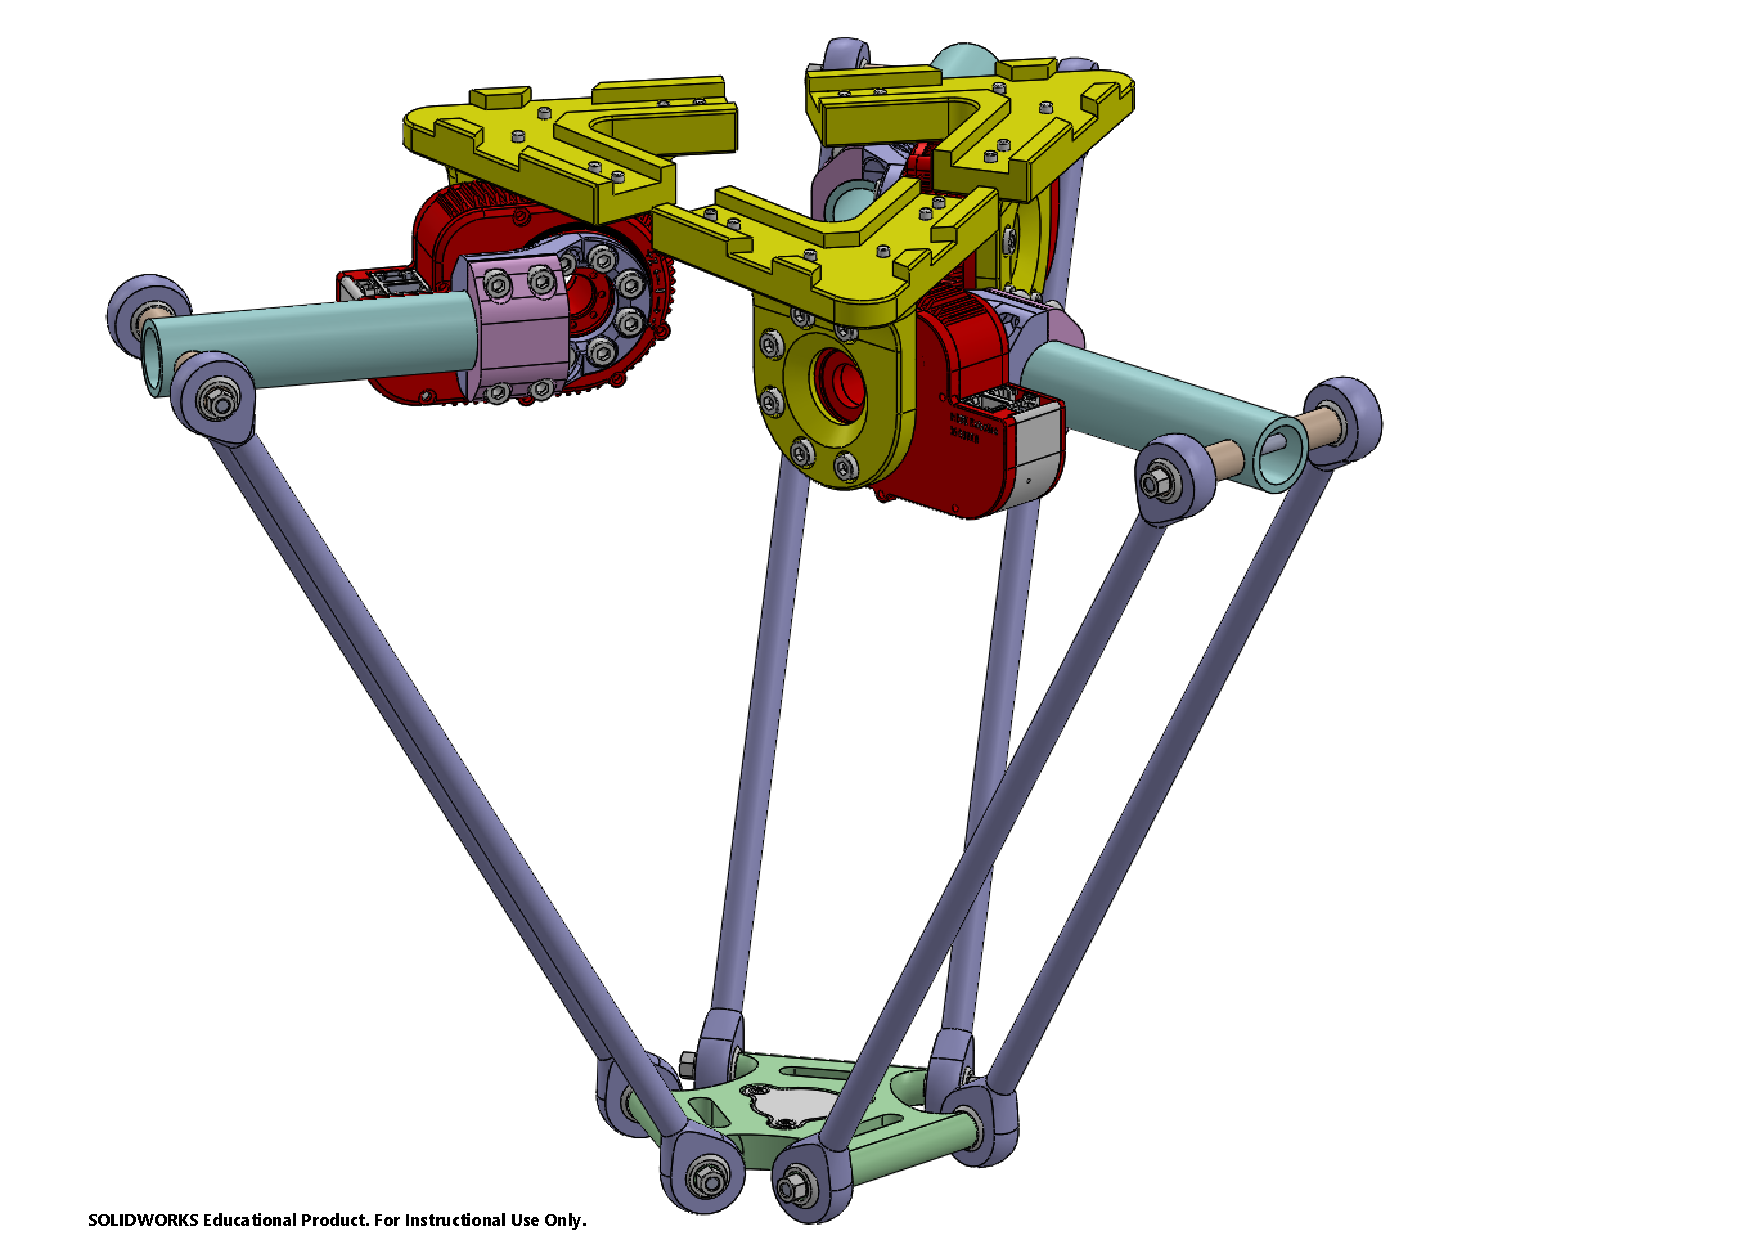
\includegraphics[width=\linewidth]{delta-unattached-dimetric-view.PDF}
      }
      \caption[Dimetrische Ansicht des unbefestigten Delta-Roboters]{Dimetrische Ansicht des unbefestigten Delta-Roboters}
      \label{fig:delta-unattached-dimetric-view}
    \end{figure}
    % \newline
    \noindent
    Der komplette Aufbau des Robotersystems ist in Abbildung \ref{fig:delta-attached-isometric-view} dargestellt. Der Rahmen zur Einhausung und der Arbeitsbereich des Roboters sind aus 20 $[mm]$ Aluminiumprofilen gefertigt, wobei für die Ebenen der Arbeitsfläche 4 $[mm]$ starke Plexiglasplatten eingesetzt werden.
    \begin{figure}[H]
      \centering
      \fbox
      {
          % 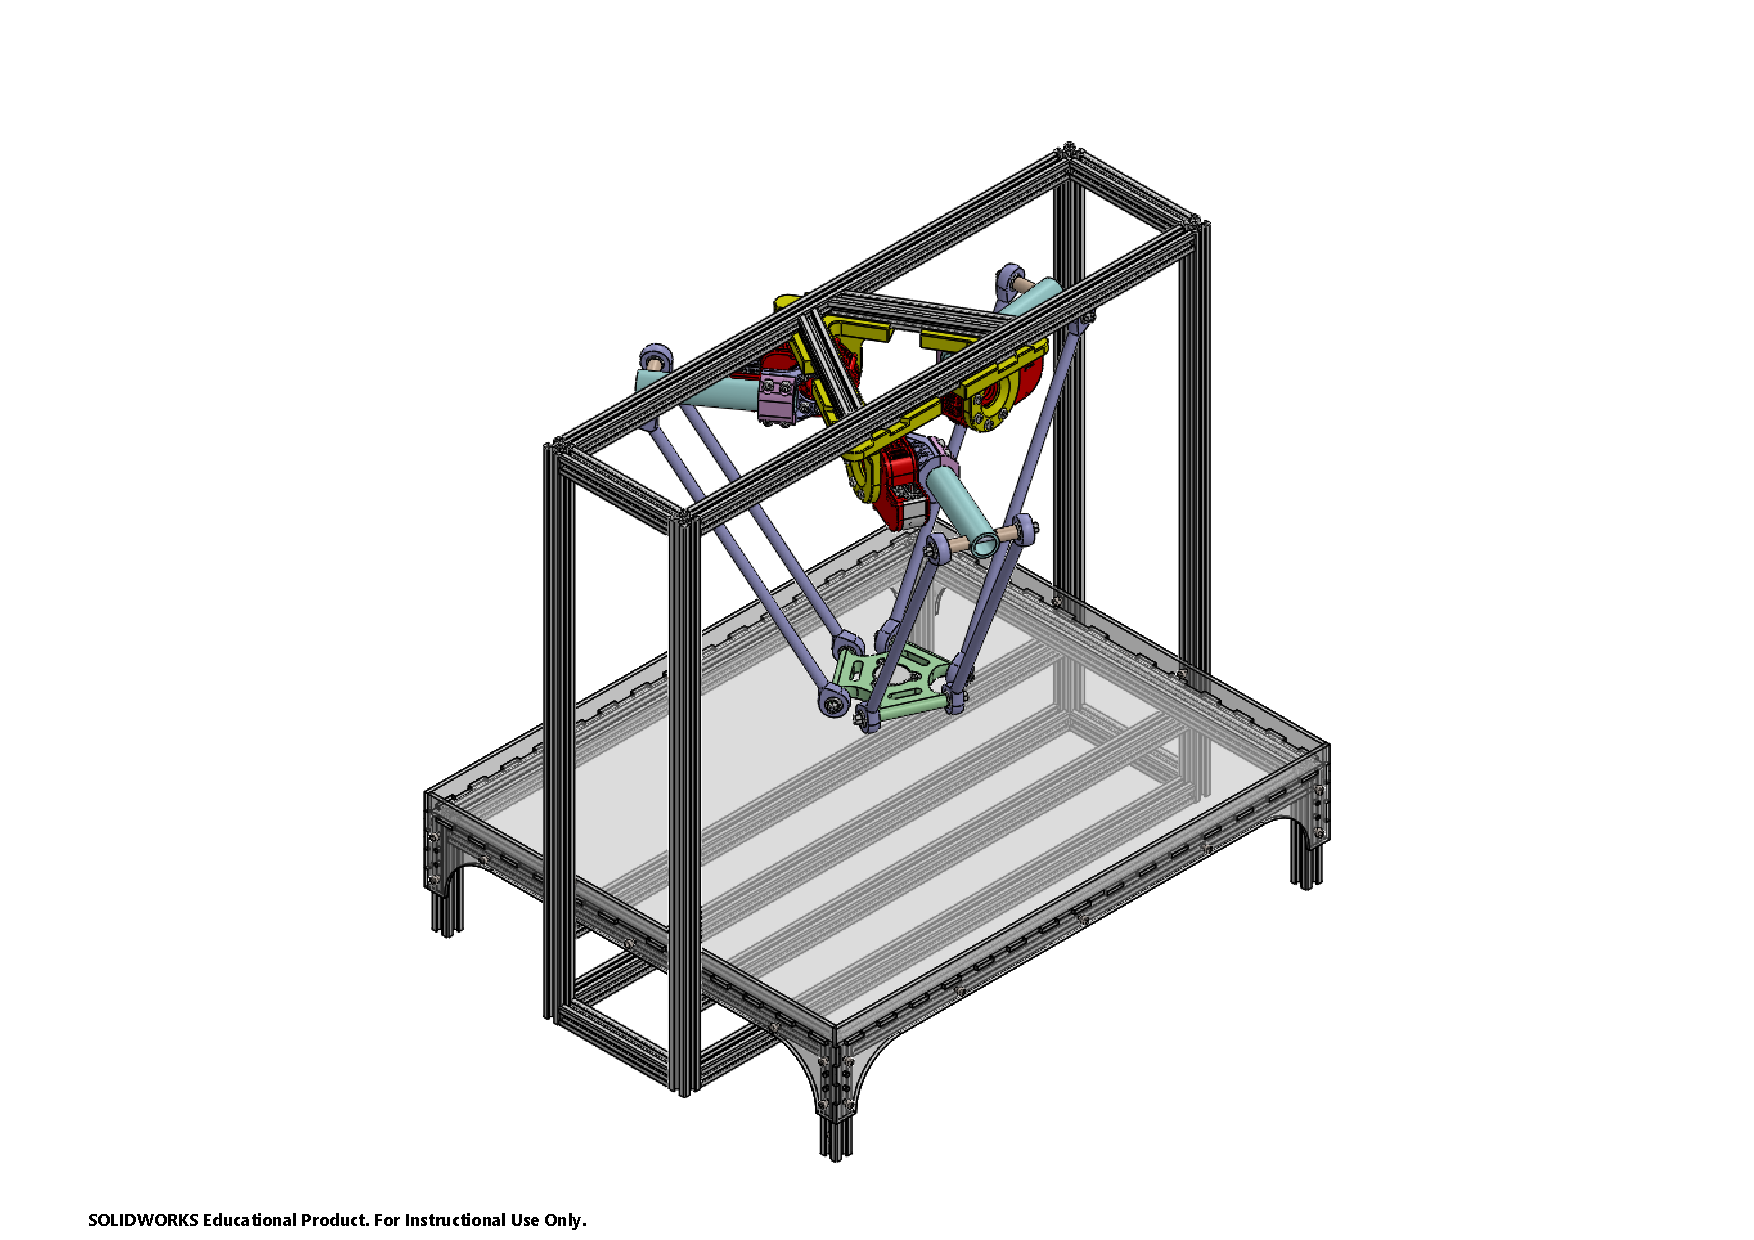
\includegraphics[width=\linewidth]{delta-attached-isometric-view.PDF}
          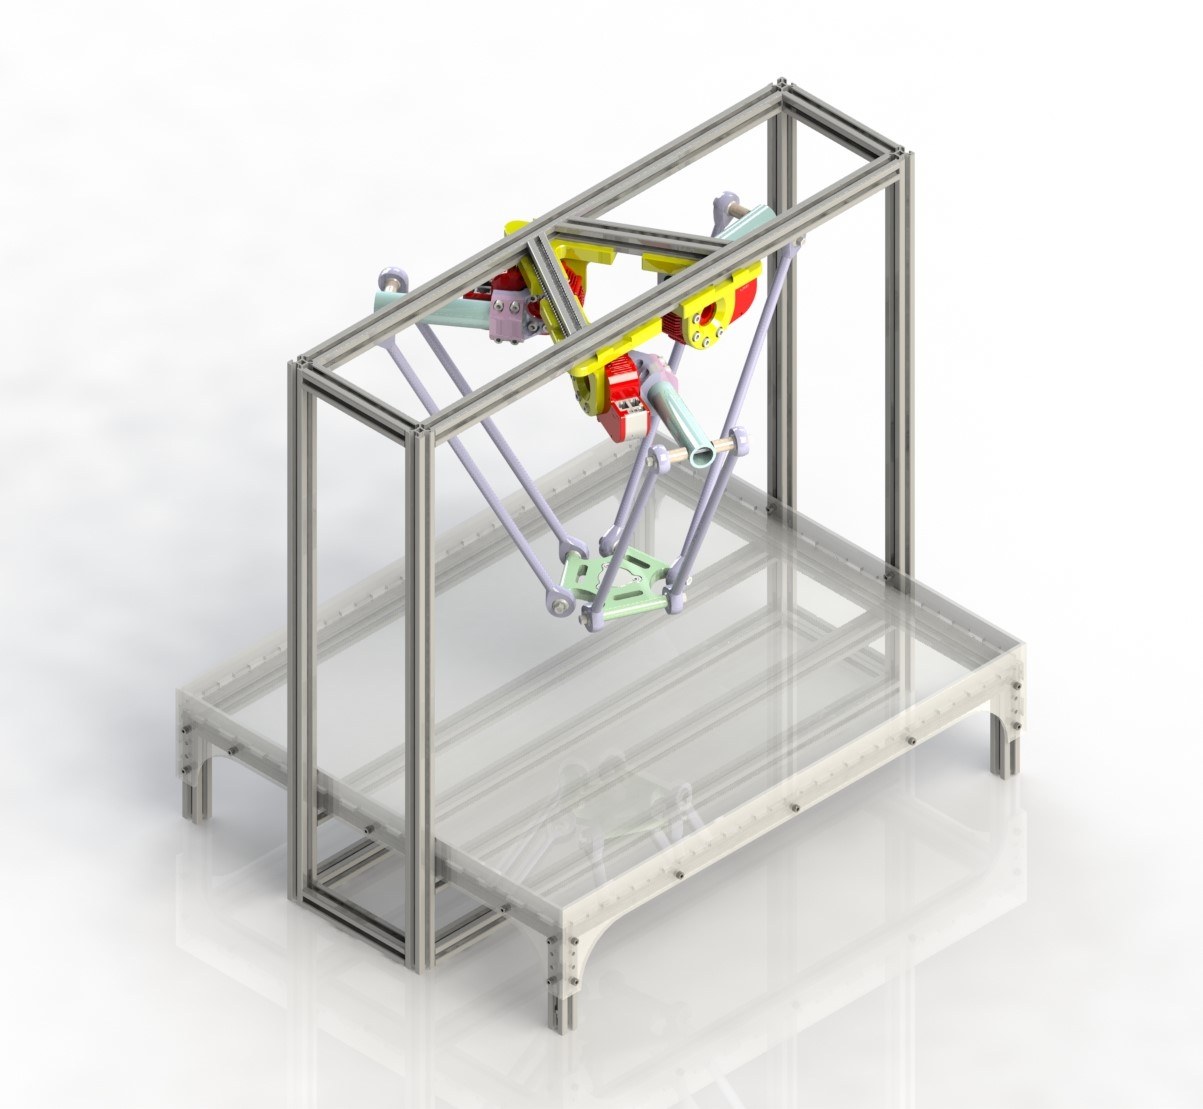
\includegraphics[width=\linewidth]{delta-attached-isometric-view-rendered-1}
      }
      \caption[Isometrische Ansicht des Delta-Roboters]{Isometrische Ansicht des Delta-Roboters}
      \label{fig:delta-attached-isometric-view}
    \end{figure}
    % \newline
    \noindent
    Die aktiven Drehgelenke des Roboters, welche die proximalen Glieder antreiben, sind über an der Basis montierte HEBI X5-1 Antriebe ausgeführt. In Abbildung \ref{fig:hebi-x5-1} ist das CAD Modell eines Aktors dargestellt. 
    \begin{figure}[H]
      \centering
      %\fbox
      {
        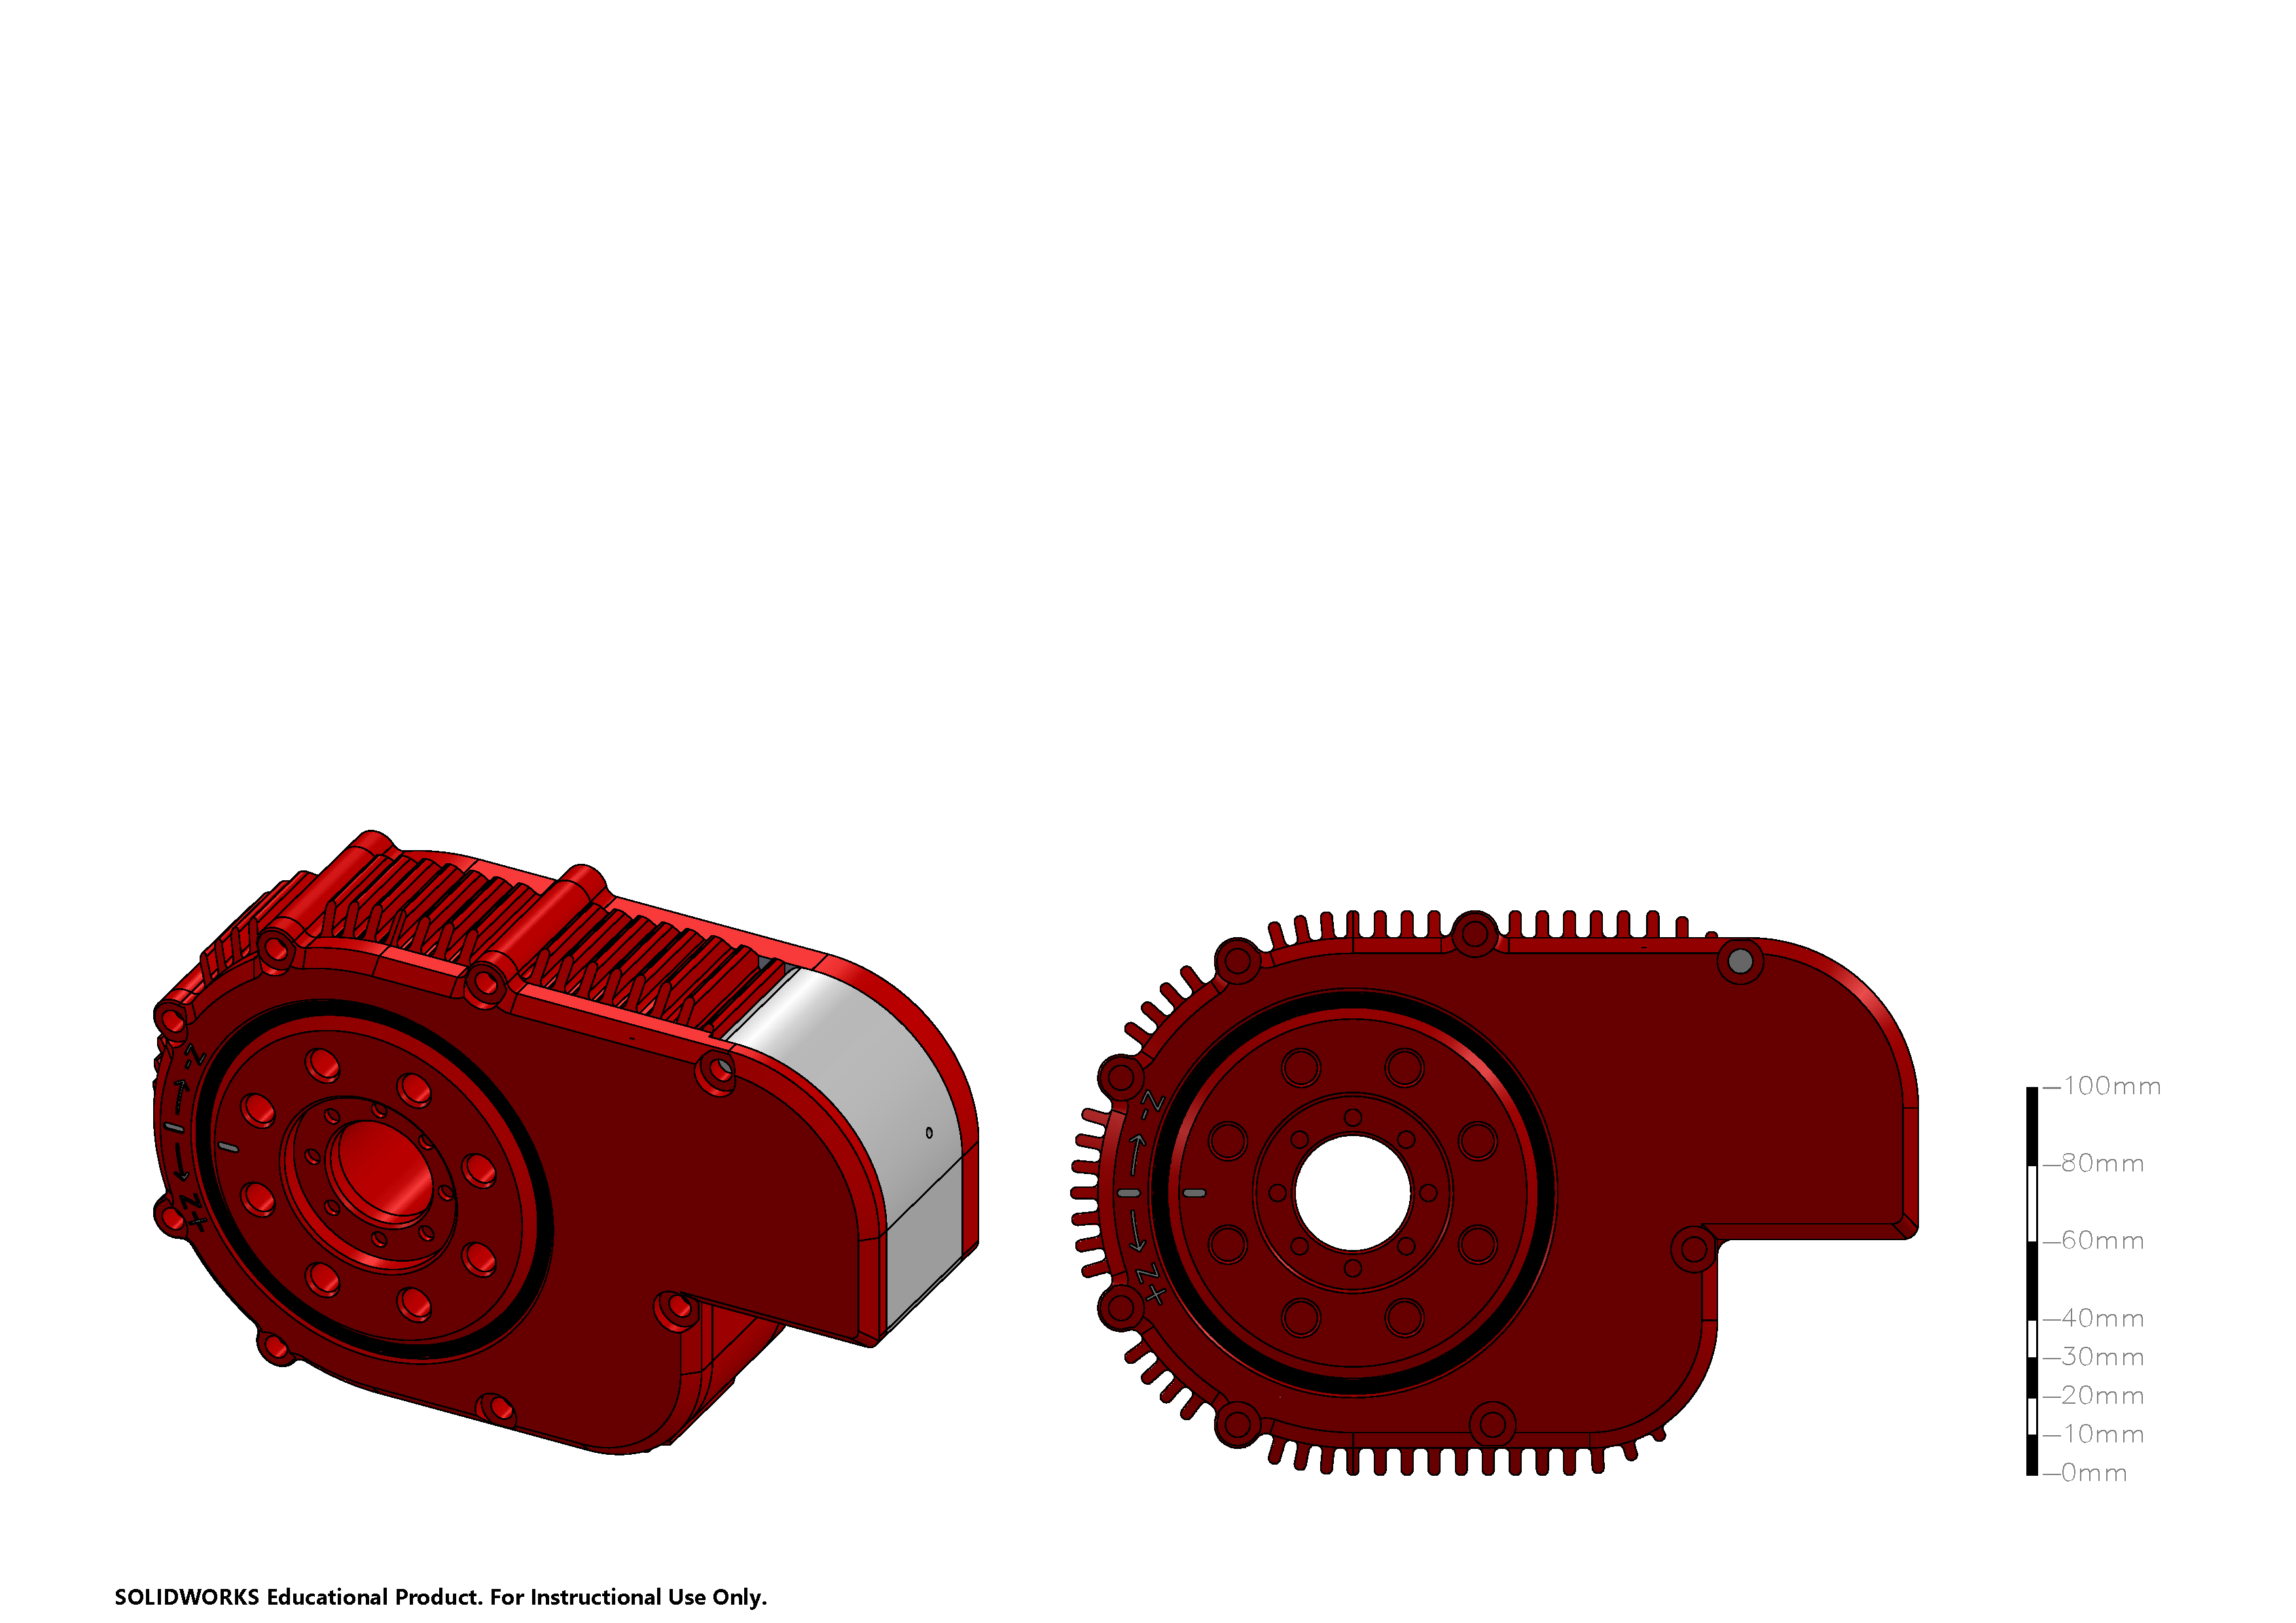
\includegraphics[width=\linewidth]{hebi-x5-1.PDF}
      }
      \caption[CAD Modell eines HEBI X5-1 Aktors]{CAD Modell eines HEBI X5-1 Aktors}
      \label{fig:hebi-x5-1}
    \end{figure}
    % \newline
    \noindent
    Da die proximalen Glieder zusätzlichen Biege- und Torsionsmomenten ausgesetzt sind, werden diese üblicherweise im Vergleich zu den distalen Gliedern stärker dimensioniert. In dieser Arbeit sind die proximalen Verbindungen über robolink\textregistered\ W Anschlussrohre aus Aluminium und die distalen Komponenten über igubal\textregistered-Doppelgelenklager KDGM der Firma IGUS realisiert. Der Aufbau eines Kugelgelenks des Doppelgelenklagers ist prädestiniert auf kleinstem Raum räumliche Schwenkbewegungen durchzuführen \cite{Ne06}. Die Energieversorgung wird über ein Mean Well GST220A24-R7B Tischnetzteil bereitgestellt. Eine detailierte Auflistung der verwendeten Komponenten kann aus Tabelle \ref{tab:stückliste} in Anhang \ref{app:stückliste} entnommen werden.\\
    \\
    Für die Inbetriebnahme der HEBI X5-1 Antriebe wird ein Ethernet-Kabel mit dem Router im lokalen Netzwerk (LAN) und dem RJ45-Port eines Antriebs verbunden. Besitzt ein Modul eine Verbindung zum Router können die restlichen Aktoren über weitere Ethernet-Kabel in Serie miteinander verbunden werden. Zusätzlich wird für die Energieversorgung jedes der Module mit einer Molex Mini-Fit Jr. Steckverbindungen an die X5/8 Stromverteilungsplatine angeschlossen, welche wiederum mit dem Netzteil verbunden ist.
    
    \section{Entwicklung der Software}
    
    Für die Entwicklung der Software wurde die von HEBI zur Verfügung gestellte MathWorks\textregistered\ MATLAB API verwendet. Die API ist freigegeben und kann in der Standard-Arbeitsumgebung von MathWorks\textregistered\ MATLAB ohne zusätzliche Add-Ons oder Toolboxes ausgeführt werden. MathWorks\textregistered\ MATLABs Fokus auf linearer Algebra und Matrixoperationen unterstützt die Roboterprogrammierung und eignet sich mit den von HEBI bereitgestellten Bibliotheken zur Modellierung komplexer Systeme, welche in Echtzeit direkt von MathWorks\textregistered\ MATLAB aus gesteuert werden können.\\
    \\
    In Scope, einer von HEBI angebotenen grafischen Benutzeroberfläche (GUI von engl. Graphical User Interface), können die Motoren überwacht und grundlegende Aufgaben, wie etwa das manuelle Senden von Befehlen, ausführen werden. Zur Absicherung werden die minimalen und maximalen Positionswerte der einzelnen Module in Scope hinterlegt. Um die Benutzerfreundlichkeit zu erhöhen sind die Steuerungsparameter der Onboard-Controller zusätzlich in einer *.XML (von engl. Extensible Markup Language) Datei abgespeichert, in der die Werte für einzelne Module sowie Modulgruppen konfiguriert, gespeichert und geladen werden können. Darüber hinaus ermöglicht ein *.HRDF (von engl. HEBI Robot Description File) das Speichern und Laden von Kinematik- und Dynamikinformationen einer Roboterkonfiguration.\\
    \\
    Die Planung der Trajektorie wird über die von HEBI zur Verfügung gestellte HebiTrajectoryGenerator API realisiert. Somit können, in Verbindung mit der Kinematik API, integrierte Schwerkraft- und Dynamikkompensationen sowie parametrisierte Bewegungen mit minimalem Ruck durchgeführt werden.

%%%%%%%%%%%%%%%%%%%%%%%%%%%%%%%%%%%%%%%%%%%%%%%%%%%%
%%        Zusammenfassung und Ausblick            %%
%%%%%%%%%%%%%%%%%%%%%%%%%%%%%%%%%%%%%%%%%%%%%%%%%%%%
\chapter{Zusammenfassung und Ausblick}
\label{cap:zusammenfassung-und-ausblick}

    In der vorliegenden Arbeit wird die mechatronische Auslegung eines Delta-Roboters für den Einsatz in der akademischen Ausbildung vorgestellt. Eine Herausforderung in der Entwicklung paralleler Robotersysteme liegt in der mathematischen Modellierung sowie in der Auslegung der Mechanik der simultan ablaufenden, räumlichen Bewegungen des Roboters.\\ 
    \\
    Um einen für Ausbildungszwecke geeigneten Roboter zu konstruieren, muss im Betriebszustand die Sicherheit für Mensch und Maschine gewährleistet werden, während aufgrund wechselnder Räumlichkeiten der Aufbau portabel gestaltet sein muss. Daraus resultieren Anforderungen einer möglichst eigensicheren, robusten Konstruktion, welche dennoch möglichst kostengünstig gefertigt werden soll. Bei der Baugröße und den Befestigungsmöglichkeiten wurde darauf geachtet, den Roboter benutzerfreundlich, kompakt und modular zu gestalten, um Erweiterungen zu ermöglichen und Wartungsarbeiten zu erleichtern.\\
    \\
    Die Arbeit beschäftigt sich anfangs mit der geometrischen und mathematischen Modellierung des Systems. Die Vorgehensweise hierfür war zunächst die Bestimmung der Freiheitsgrade sowie die Berechnung des Modells der inversen Kinematik des Delta-Roboters. Nach erfolgreichem Abschluss der Konzeptionsphase wurde anschließend ein Prototyp des Delta-Roboters konstruiert und programmiert, um das entworfene Modell am Testaufbau auf Richtigkeit überprüfen zu können. Als Fertigungsverfahren wurde hierbei Rapid Prototyping eingesetzt.\\ 
    \\
    Die Steuerungsarchitektur, welche in MathWorks\textregistered\ MATLAB mithilfe der von HEBI zur Verfügung gestellten MathWorks\textregistered\ MATLAB API numerisch implementiert wurde, umfasst das Modell der inversen Kinematik. Die Ergebnisse bestätigen die Funktionsfähigkeit der Algorithmen und zeigen, dass das System wie erwartet bei bekannter Pose des Endeffektors die entsprechenden Gelenkwinkel liefert und der Steuerung zur Trajektorienplanung übergibt. Systemtests wurden in Scope, einer von HEBI angebotenen GUI zur Überwachung der Motoren und zum Senden manueller Befehle, durchgeführt. In der GUI wurden auch die minimalen und maximalen Positionswerte der einzelnen Module zur Absicherung hinterlegt.\\
    \\
    Den Abschluss der Arbeit bildet die \textit{Jacobi-Matrix} der Kinematik, welche basierend auf dem Modell der inversen Kinematik bestimmt wird. Diese beschreibt den Zusammenhang zwischen den Gelenkgeschwindigkeiten und der Geschwindigkeit des Endeffektors im kartesischen Raum und dient als Grundlage für Singularitätsuntersuchungen und dynamische Berechnungen des Roboters.\\
    \\
    Die Ergebnisse zeigen, dass ein Prototyp für didaktische Zwecke in der akademischen Ausbildung eigensicher, transportabel und kostengünstig hergestellt werden kann, um angehenden Ingenieuren die einzigartige Möglichkeit zu bieten, parallelkinematische Maschinen praxisorientiert zu studieren. Zusammengefasst kann gesagt werden, dass die vorliegende Arbeit das gewünschte Ziel, die mechatronische Auslegung eines Delta-Roboters für den Einsatz in der akademischen Ausbildung zu entwickeln, erfüllt.\\
    \\
    Im Ausblick für den akademischen Einsatz des Systems können präzise Konstruktionsauslegungen mit Hilfe der inversen Kinematik evaluiert werden, um in weiterführenden Arbeiten Fertigungs- und Montagetoleranzen optimieren und infolgedessen die Positionier- und Wiederholgenauigkeit des Delta-Roboters verbessern zu können. Zusätzlich können über die \textit{Jacobi-Matrix} Singularitätsuntersuchungen durchgeführt werden, um bei Studierenden ein besseres Verständnis der Thematik zu schaffen. Weitere Verbesserungsmöglichkeiten des Aufbaus werden im folgenden Kapitel \ref{cap:diskussion} diskutiert.


%%%%%%%%%%%%%%%%%%%%%%%%%%%%%%%%%%%%%%%%%%%%%%%%%%%%
%%                  Diskussion                    %%
%%%%%%%%%%%%%%%%%%%%%%%%%%%%%%%%%%%%%%%%%%%%%%%%%%%%
\chapter{Diskussion}
\label{cap:diskussion}

    Die Auslegung und Entwicklung von Robotersystemen erfordert eine hohe Erfahrung von Seiten der Entwickler. Auch wenn die vorliegende Arbeit das gewünschte Ziel, die mechatronische Auslegung und Entwicklung eines Delta-Roboters für den Einsatz in der akademischen Ausbildung, erfüllt, gibt es dennoch umfangreiche Verbesserungspotenziale.\\
    \\
    Unter anderem hat die verwendete Regelungsstrategie große Auswirkungen auf das dynamische Verhalten des Roboters. Wie ein Aktuator auf Befehle reagiert, hängt von der gewählten Regelungsstrategie des Moduls ab. Die Steuerung und Abstimmung von Aktuatoren ist ein komplexes Thema. HEBI stellt diesbezüglich eine vorkonfigurierte, gebrauchsfertige Regelungsstrategie zur Verfügung, welche bei geringer Belastung eine gute Leistung erbringt. Bei schweren Lasten und komplexen Systemen mit mehreren Freiheitsgraden muss diese jedoch wahrscheinlich auf die spezifische Anwendung abgestimmt werden. In der Arbeit wurde die von HEBI eingerichtete Regelungsstrategie verwenden, während des Betriebs waren jedoch deutliche Schwingungen bemerkbar. Folglich könnte zur Abhilfe in weiterführenden Arbeiten eine angemessene Regelung und Trajektorienplanung ausgelegt und entworfen werden, um die Positionier- und Wiederholgenauigkeit des Roboters zu erhöhen und einen präzisen Pfad zu erreichen.\\
    \\
    Um die Positionier- und Wiederholgenauigkeit des Roboters zu erhöhen gibt es einige weiter verfolgbare Verbesserungsansätze. Die oben genannte Regelungsstrategie spielt in diesem Zusammenhang eine ausschlaggebende Rolle, aber auch die Fertigungs- und Montagetoleranzen der mechanischen Struktur haben großen Einfluss. Auswirkungen der ungenauen Fertigungsverfahren machen sich im Spiel der Lager und Verbindungen bemerkbar, da weder der Arbeitsbereich des Roboters noch die invariante Plattform zu der von x und y aufgespannten Ebene vollkommen parallel liegen. Die SLS gedruckten Teile weisen hierbei angemessene Eigenschaften auf, die FFF 3D-Druck Teile und die händisch durchbohrten Aluminiumrohre der proximalen Glieder besitzen jedoch schlechte Maßgenauigkeit. Als Maßnahme könnten die Gelenkverbindungen zwischen den proximalen und distalen Gliedern sowohl kraft- als auch formschlüssig ausgeführt werden. Die Doppelgelenklager der distalen Glieder könnten zudem durch höherwertige Lager mit größerem Kippwinkel ersetzten werden, was jedoch auch negative Auswirkungen auf die Kosten des Systems mit sich bringen würde.\\ 
    \\
    Um den Delta-Roboter als kartesische Positioniereinrichtung mit drei DoF in x, y und z-Richtung verwenden zu können sind lineare Bewegungen mit definierter z-Höhe auf einer von x und y aufgespannten Ebene unerlässlich. Die Linearisierung der Pfade wurde in der Trajektorienplanung in MathWorks\textregistered\ MATLAB, mithilfe der von HEBI zur Verfügung gestellten API, erstellt. Hierbei können die verwendeten Algorithmen in weiterführenden Arbeiten zeitoptimiert werden, indem etwa die Verwendung von Schleifen vermieden wird. Zudem kann das Programm zuverlässiger und robuster gestaltet sowie mit weiteren Funktionen ergänzt werden.\\
    \\
    Voraussetzung für die Weiterentwicklung des Roboters und weitere Vorgehensweise zur Optimierung der Kinematik könnten eine Arbeitsraumanalyse umfassen. Darüber hinaus könnte mithilfe der \textit{Jacobi-Matrix} eine Singularitätsuntersuchung sowie eine dynamische Modellierung des Roboters, etwa nach dem Lagrange oder Newton–Euler Verfahren, durchgeführt werden, um eine Grundlage für die Auslegung und den Entwurf einer Regelung und Trajektorienplanung zu erhalten. 
    % Verbesserungspotenziale:
    % \begin{itemize} 
    %     \item Regelungsverfahren der Antriebe
    %     \item Pfadplanung (Linearisierung) 
    %     \item Schlechte Positionier- und Wiederholgenauigkeit. Dennoch: Die Implementierung des inversen kinematischen Modells bestätigt die Funktionsfähigkeit der Algorithmen.
    %     \item Fertigungsverfahren:
    %         \begin{itemize} 
    %             \item Fertigungs- und Montagetoleranzen in der mechanischen Struktur
    %                 \begin{itemize}
    %                     \item Tisch: nicht parallel
    %                     \item Plattform: nicht parallel
    %                 \end{itemize}
    %             \item SLS für Verbindungen: angemessen
    %             \item Distale Glieder: Doppelgelenklager durch höherwertige/leichtgängigere mit größerem Kippwinkel ersetzten
    %             \item Gelenkverbindung zwischen proximalen und distalen Gliedern: nicht optimal (Form- und Kraftschlüssig?)
    %         \end{itemize}
    % \end{itemize}
    % Weitere Vorgehensweise zur Optimierung der Kinematik, Voraussetzung für die Weiterentwicklung des Roboters:
    % \begin{itemize}
    %     \item Arbeitsraumanalyse
    %     \item Fertigungs- und Montagetoleranz optimieren
    %     \item Singularitätsuntersuchung durchführen
    %     \item Dynamische Modellierung des Roboters (etwa nach dem Lagrange oder Newton–Euler Verfahren) durchführen
    %     \item Regelung und Trajektorienplanung optimieren (Auslegung und dem Entwurf einer geeigneten Regelung)
    % \end{itemize}

% --------------------------------------------------
% BIBLIOGRAPHY
% --------------------------------------------------
\newpage
\ifthenelse{\equal{\FHTWCitationType}{HARVARD}}{}{\bibliographystyle{gerabbrv}}
\bibliography{References}
\clearpage


% --------------------------------------------------
% GLOSSARIES
% --------------------------------------------------
% Das Abbildungsverzeichnis
\listoffigures
\clearpage

% Das Tabellenverzeichnis
\listoftables
\clearpage

% Das Quellcodeverzeichnis
% \listofcode
% \clearpage

% Das Formelverzeichnis
\listofequations
\clearpage

\phantomsection
\addcontentsline{toc}{chapter}{\listacroname}
\chapter*{\listacroname}
\begin{acronym}[XXXXX]
    \acro{API}[API]{von engl. Application Programming Interface (Programmierschnittstelle)}
    \acro{CAD}[CAD]{von engl. Computer-Aided Design (Rechnerunterstütztes Konstruieren)}
    \acro{DoF}[DoF]{von engl. Degree of Freedom (Freiheitsgrad)}
    \acro{FFF}[FFF]{von engl. Fused Filament Fabrication (Schmelzschichtung)}
    \acro{GUI}[GUI]{von engl. Graphical User Interface (Grafische Benutzeroberfläche)}
    \acro{HRDF}[HRDF]{von engl. HEBI Robot Description File (HEBI Roboter Beschreibungs Datei)}
    \acro{IoT}[IoT]{von engl. Internet of Things (Internet der Dinge)}
    \acro{LAN}[LAN]{von engl. Local Area Network (Lokales Netzwerk)}
    \acro{MATLAB}[MATLAB]{von engl. MATrix LABoraty}
    \acro{ROS}[ROS]{von engl. Robot Operating System}
    \acro{SLS}[SLS]{Selektives Lasersintern}
    \acro{TCP}[TCP]{von engl. Tool Center Point (Arbeitspunkt am Ende der kinematischen Kette)}
    \acro{XML}[XML]{von engl. Extensible Markup Language (Erweiterbare Auszeichnungssprache)}
\end{acronym}


% --------------------------------------------------
% APPENDIX
% --------------------------------------------------
\newpage
\appendix

\clearpage   
\chapter{Stückliste}
\label{app:stückliste}

    \begin{table}[!htbp]
        \centering
        \caption{Stückliste}\label{tab:stückliste}
            
            \begin{tabular}{| l | c |}\hline \rowcolor[gray]{0.8}
                Beschreibung & Anzahl\\\hline
                
                HEBI X5-1 Motoren & 3\\\hline
                Gewindestange M5 110 [mm] & 6\\\hline
                Aluprofil 20x20 600 [mm] & 10\\\hline
                Aluprofil 20x20 550 [mm] und 452 [mm] und 152 [mm] & 2\\\hline
                % Aluprofil 20x20  & 2\\\hline
                Aluprofil 20x20 132 [mm] und 120 [mm] & 4\\\hline
                % Aluprofil 20x20  & 2\\\hline
                % Aluprofil 20x20  & 4\\\hline
                Aluwinkel 20x20 [mm] & 40\\\hline
                Verbindungszapfen (SLS) & 6\\\hline
                Drehgelenkverbindung (SLS) & 3\\\hline
                Gelenkgegenstück (SLS) & 3\\\hline
                Basisverbindung (SLS) & 3\\\hline
                Flansch und Kalibrierungspin (SLS) & 1\\\hline
                %  (SLS) & 1\\\hline
                Igubal\textregistered-Doppelgelenklager KDGM & 6\\\hline
                Robolink\textregistered\ W Anschlussrohren aus Aluminium 137.5 [mm] & 3\\\hline
                Mean Well GST220A24-R7B Tischnetzteil & 1\\\hline 
                X5/8 Stromverteilungsplatine & 1\\\hline
                %  & 98\\\hline
                M5 x 10 Zylinderkopfschrauben & 36\\\hline
                M5 x 16 Zylinderkopfschrauben und M5 Muttern & 12\\\hline
                M4 x 10 Zylinderkopfschrauben und 6 M4 Nutmuttern & 98\\\hline
                M3 x 10 Zylinderkopfschrauben und M3 Muttern & 3\\\hline
                % M5 Muttern & 48\\\hline
                %  & 12\\\hline
                %  & 3\\\hline
                Plexiglas 60x80 [mm] & 1\\\hline
                \end{tabular}
    \end{table}

\clearpage  
\chapter{CAD Modell des Roboters}
\label{app:cad}
    
    % \begin{figure}[ht]
    %   \centering
    %   \includegraphics[width=\linewidth]{delta-attached-side-view.PDF}
    %   \caption[Seitenansicht des befestigten Delta-Roboters.]{Seitenansicht des befestigten Delta-Roboters.}
    %   \label{fig:delta-attached-side-view}
    % \end{figure}
    
    \begin{figure}[ht]
      \centering
      %\fbox
      {
        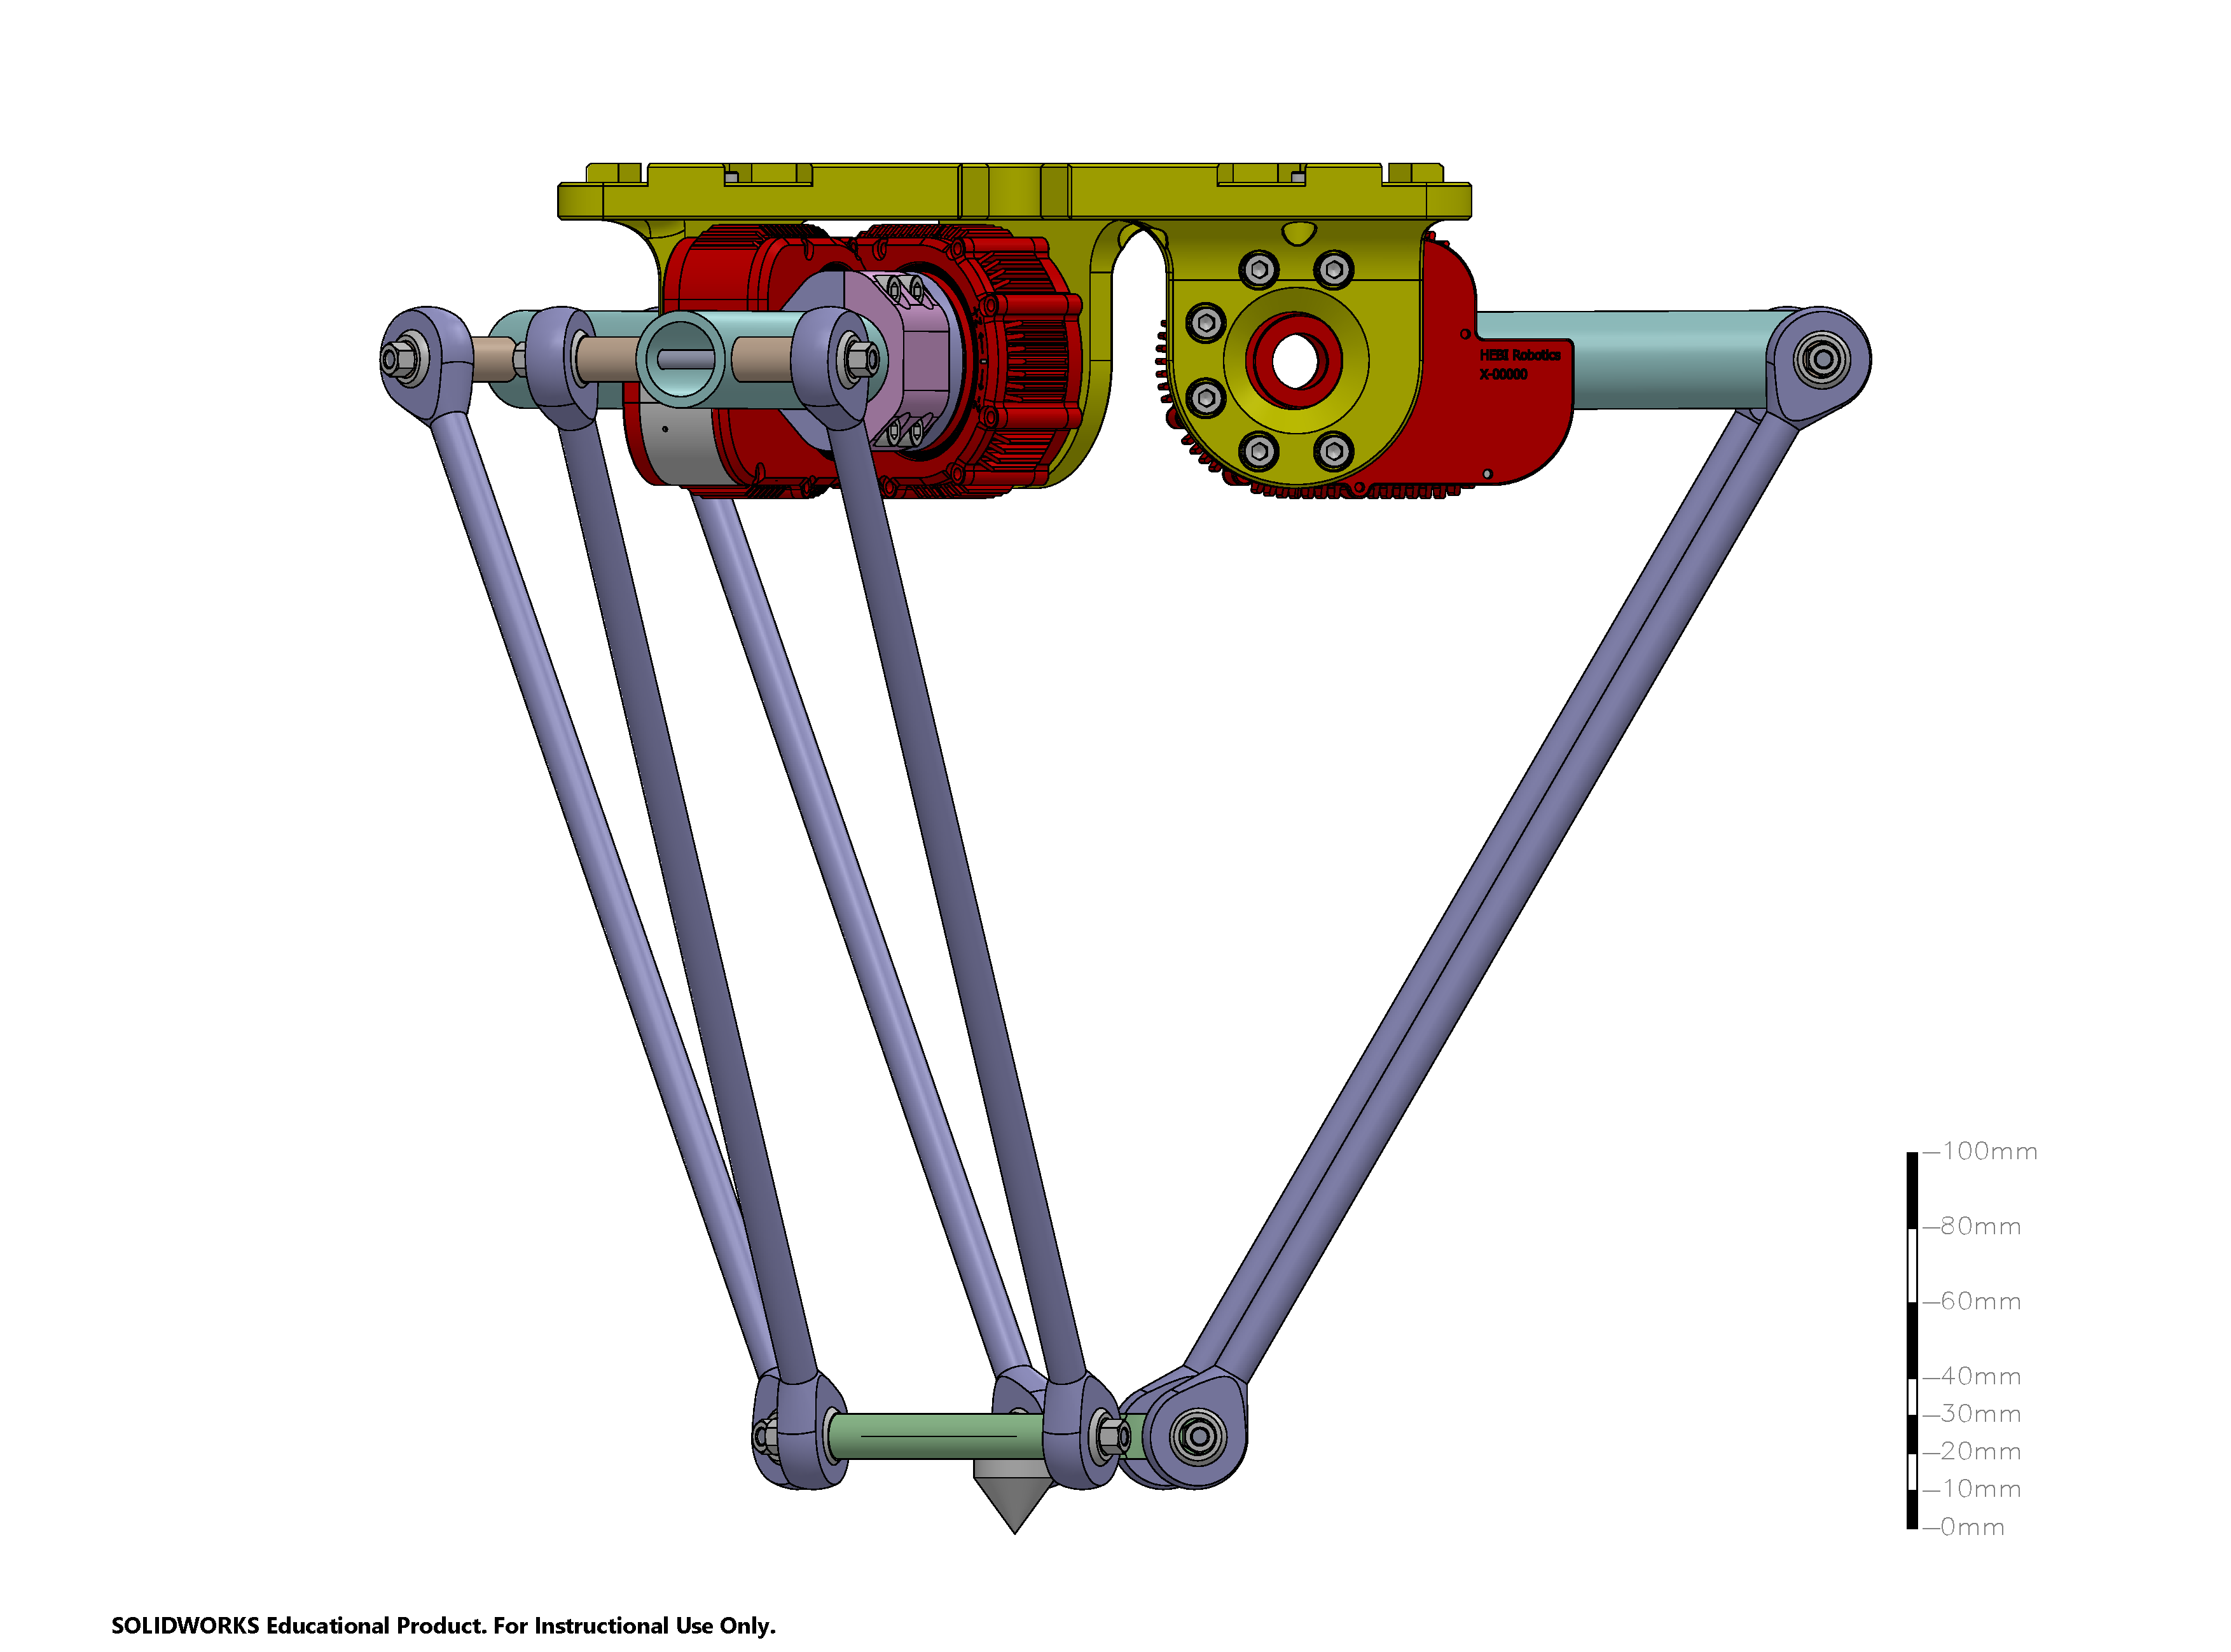
\includegraphics[width=\linewidth]{delta-unattached-side-view.PDF}
      }
      \caption[Seitenansicht des Delta-Roboters]{Seitenansicht des Delta-Roboters}
      \label{fig:delta-side-view}
    \end{figure}
    
    \begin{figure}[ht]
      \centering
      %\fbox
      {
          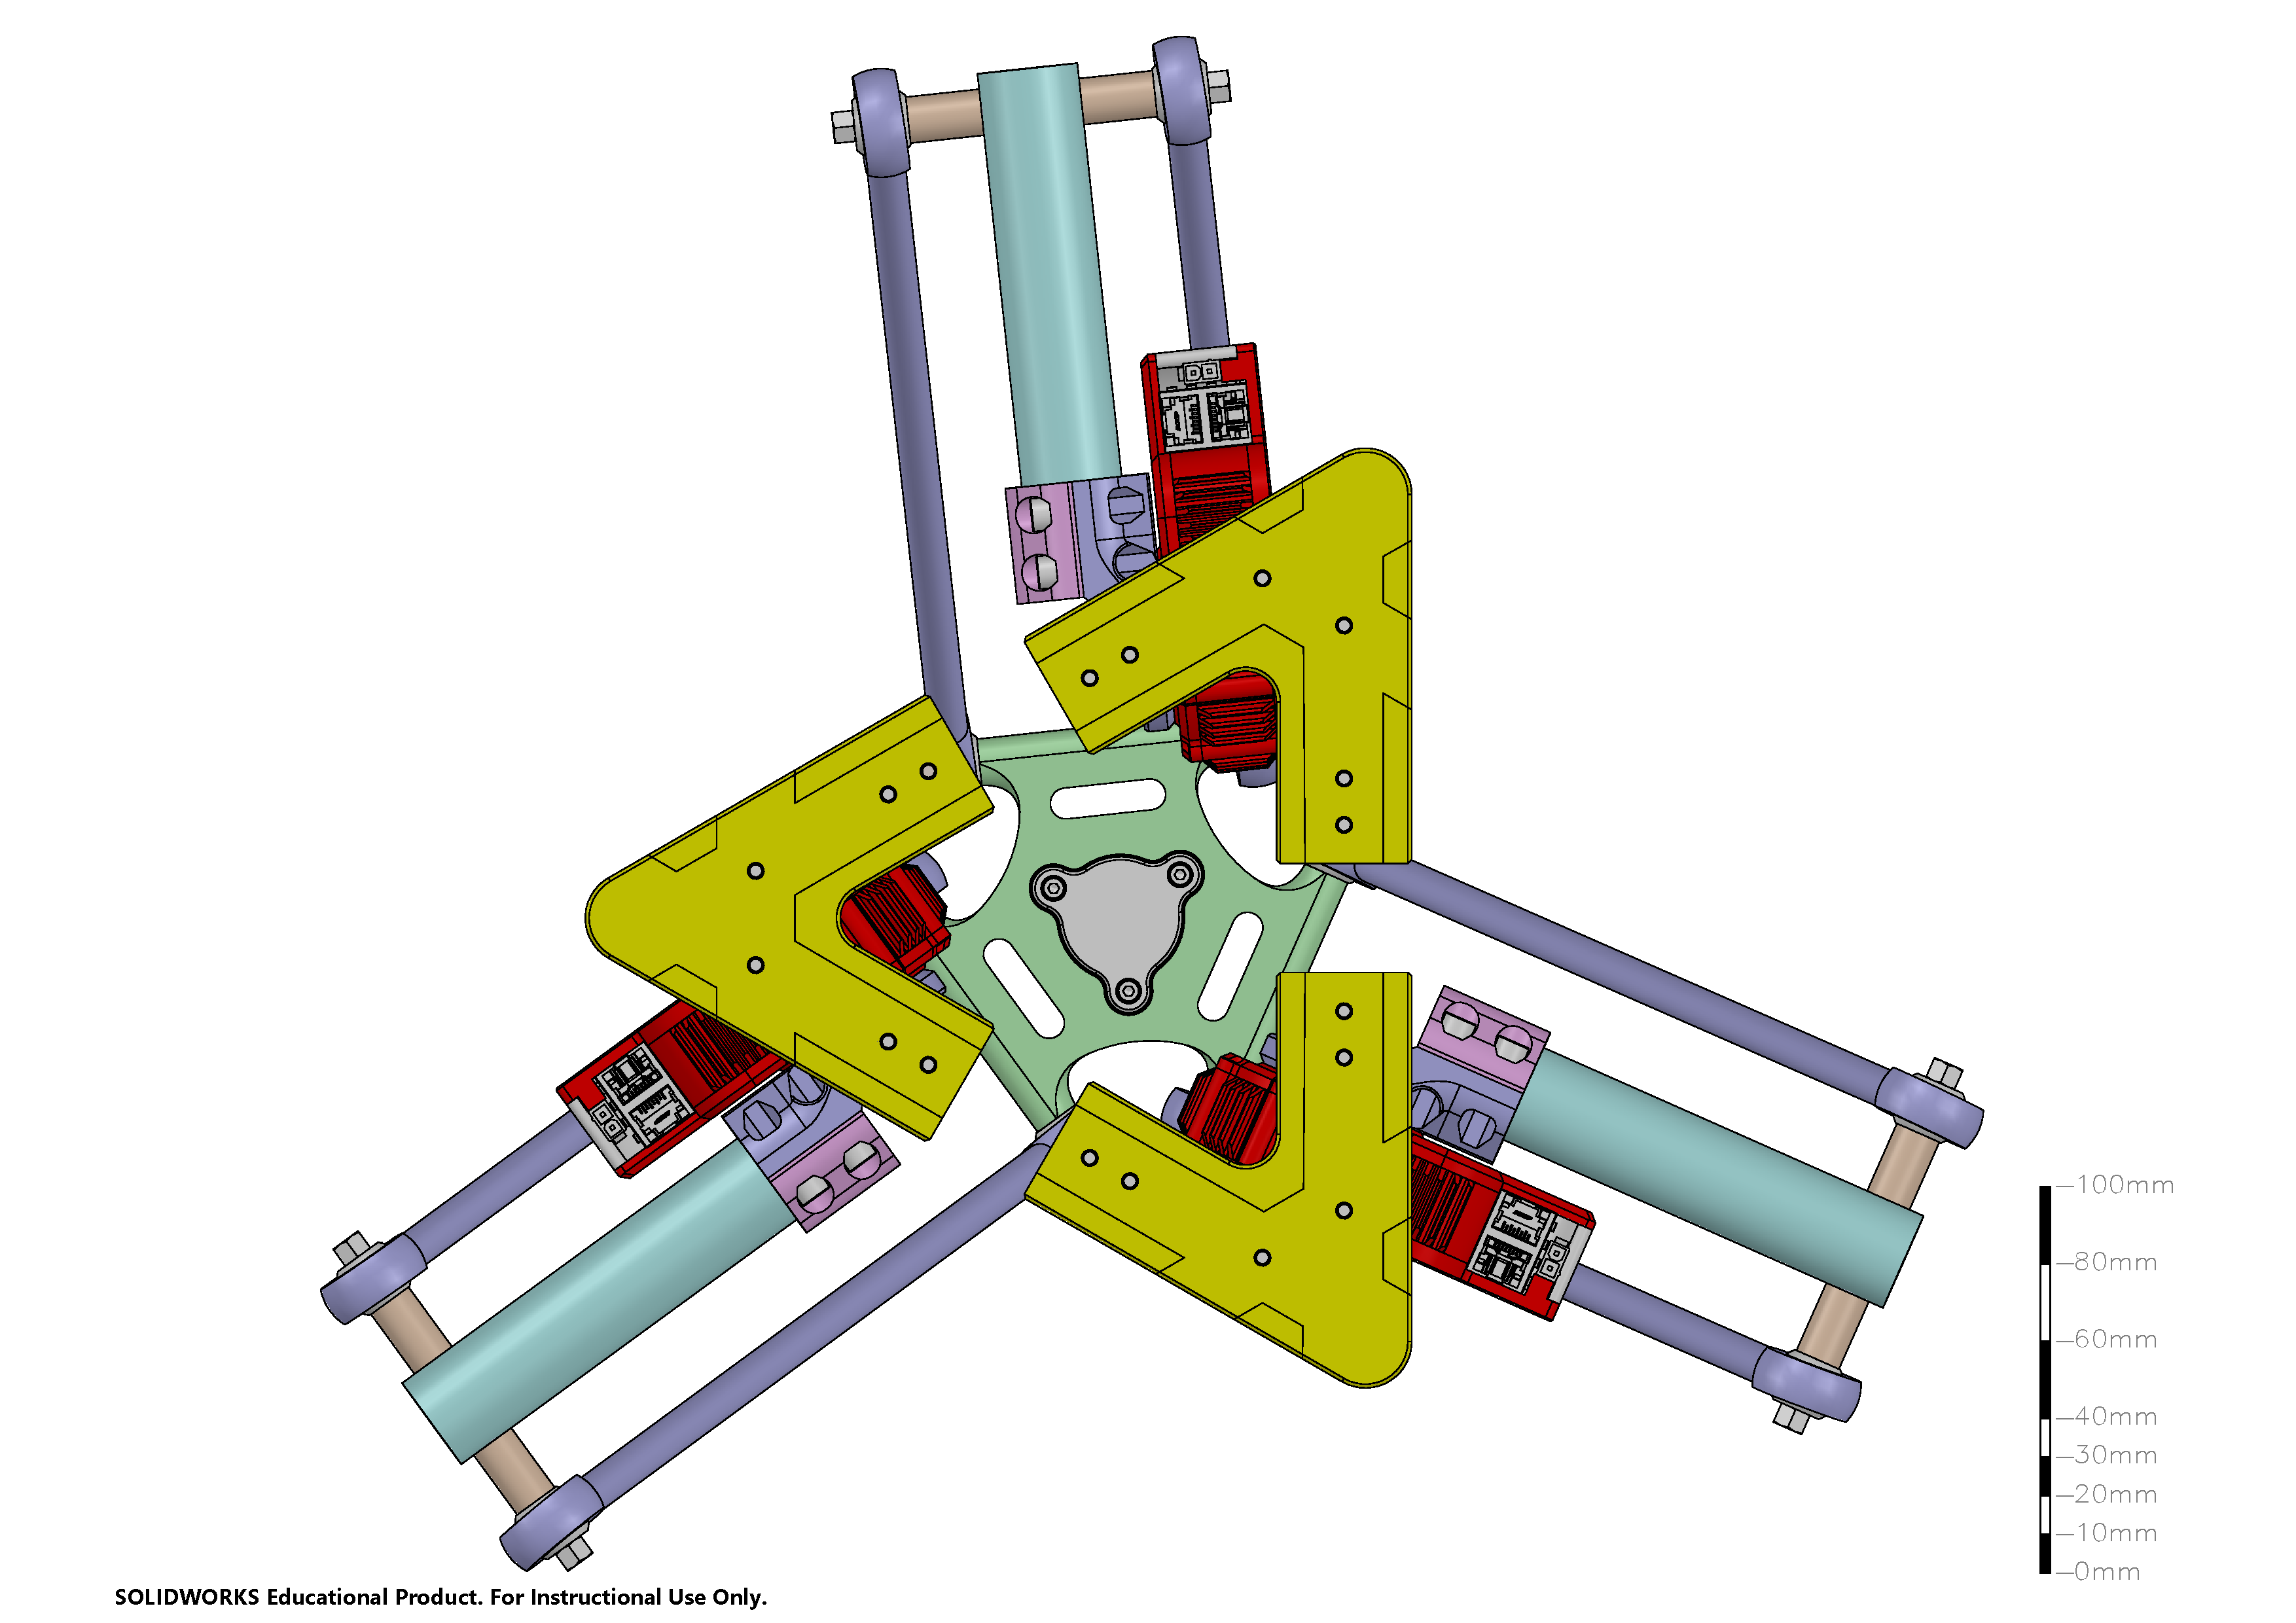
\includegraphics[width=\linewidth]{delta-unattached-top-view.PDF}
          % \includegraphics[width=\linewidth]{delta-attached-top-view.PDF}
      }
      \caption[Draufsicht des Delta-Roboters]{Draufsicht des Delta-Roboters}
      \label{fig:delta-top-view}
    \end{figure}
    
    % \begin{figure}[ht]
    %   \centering
    %   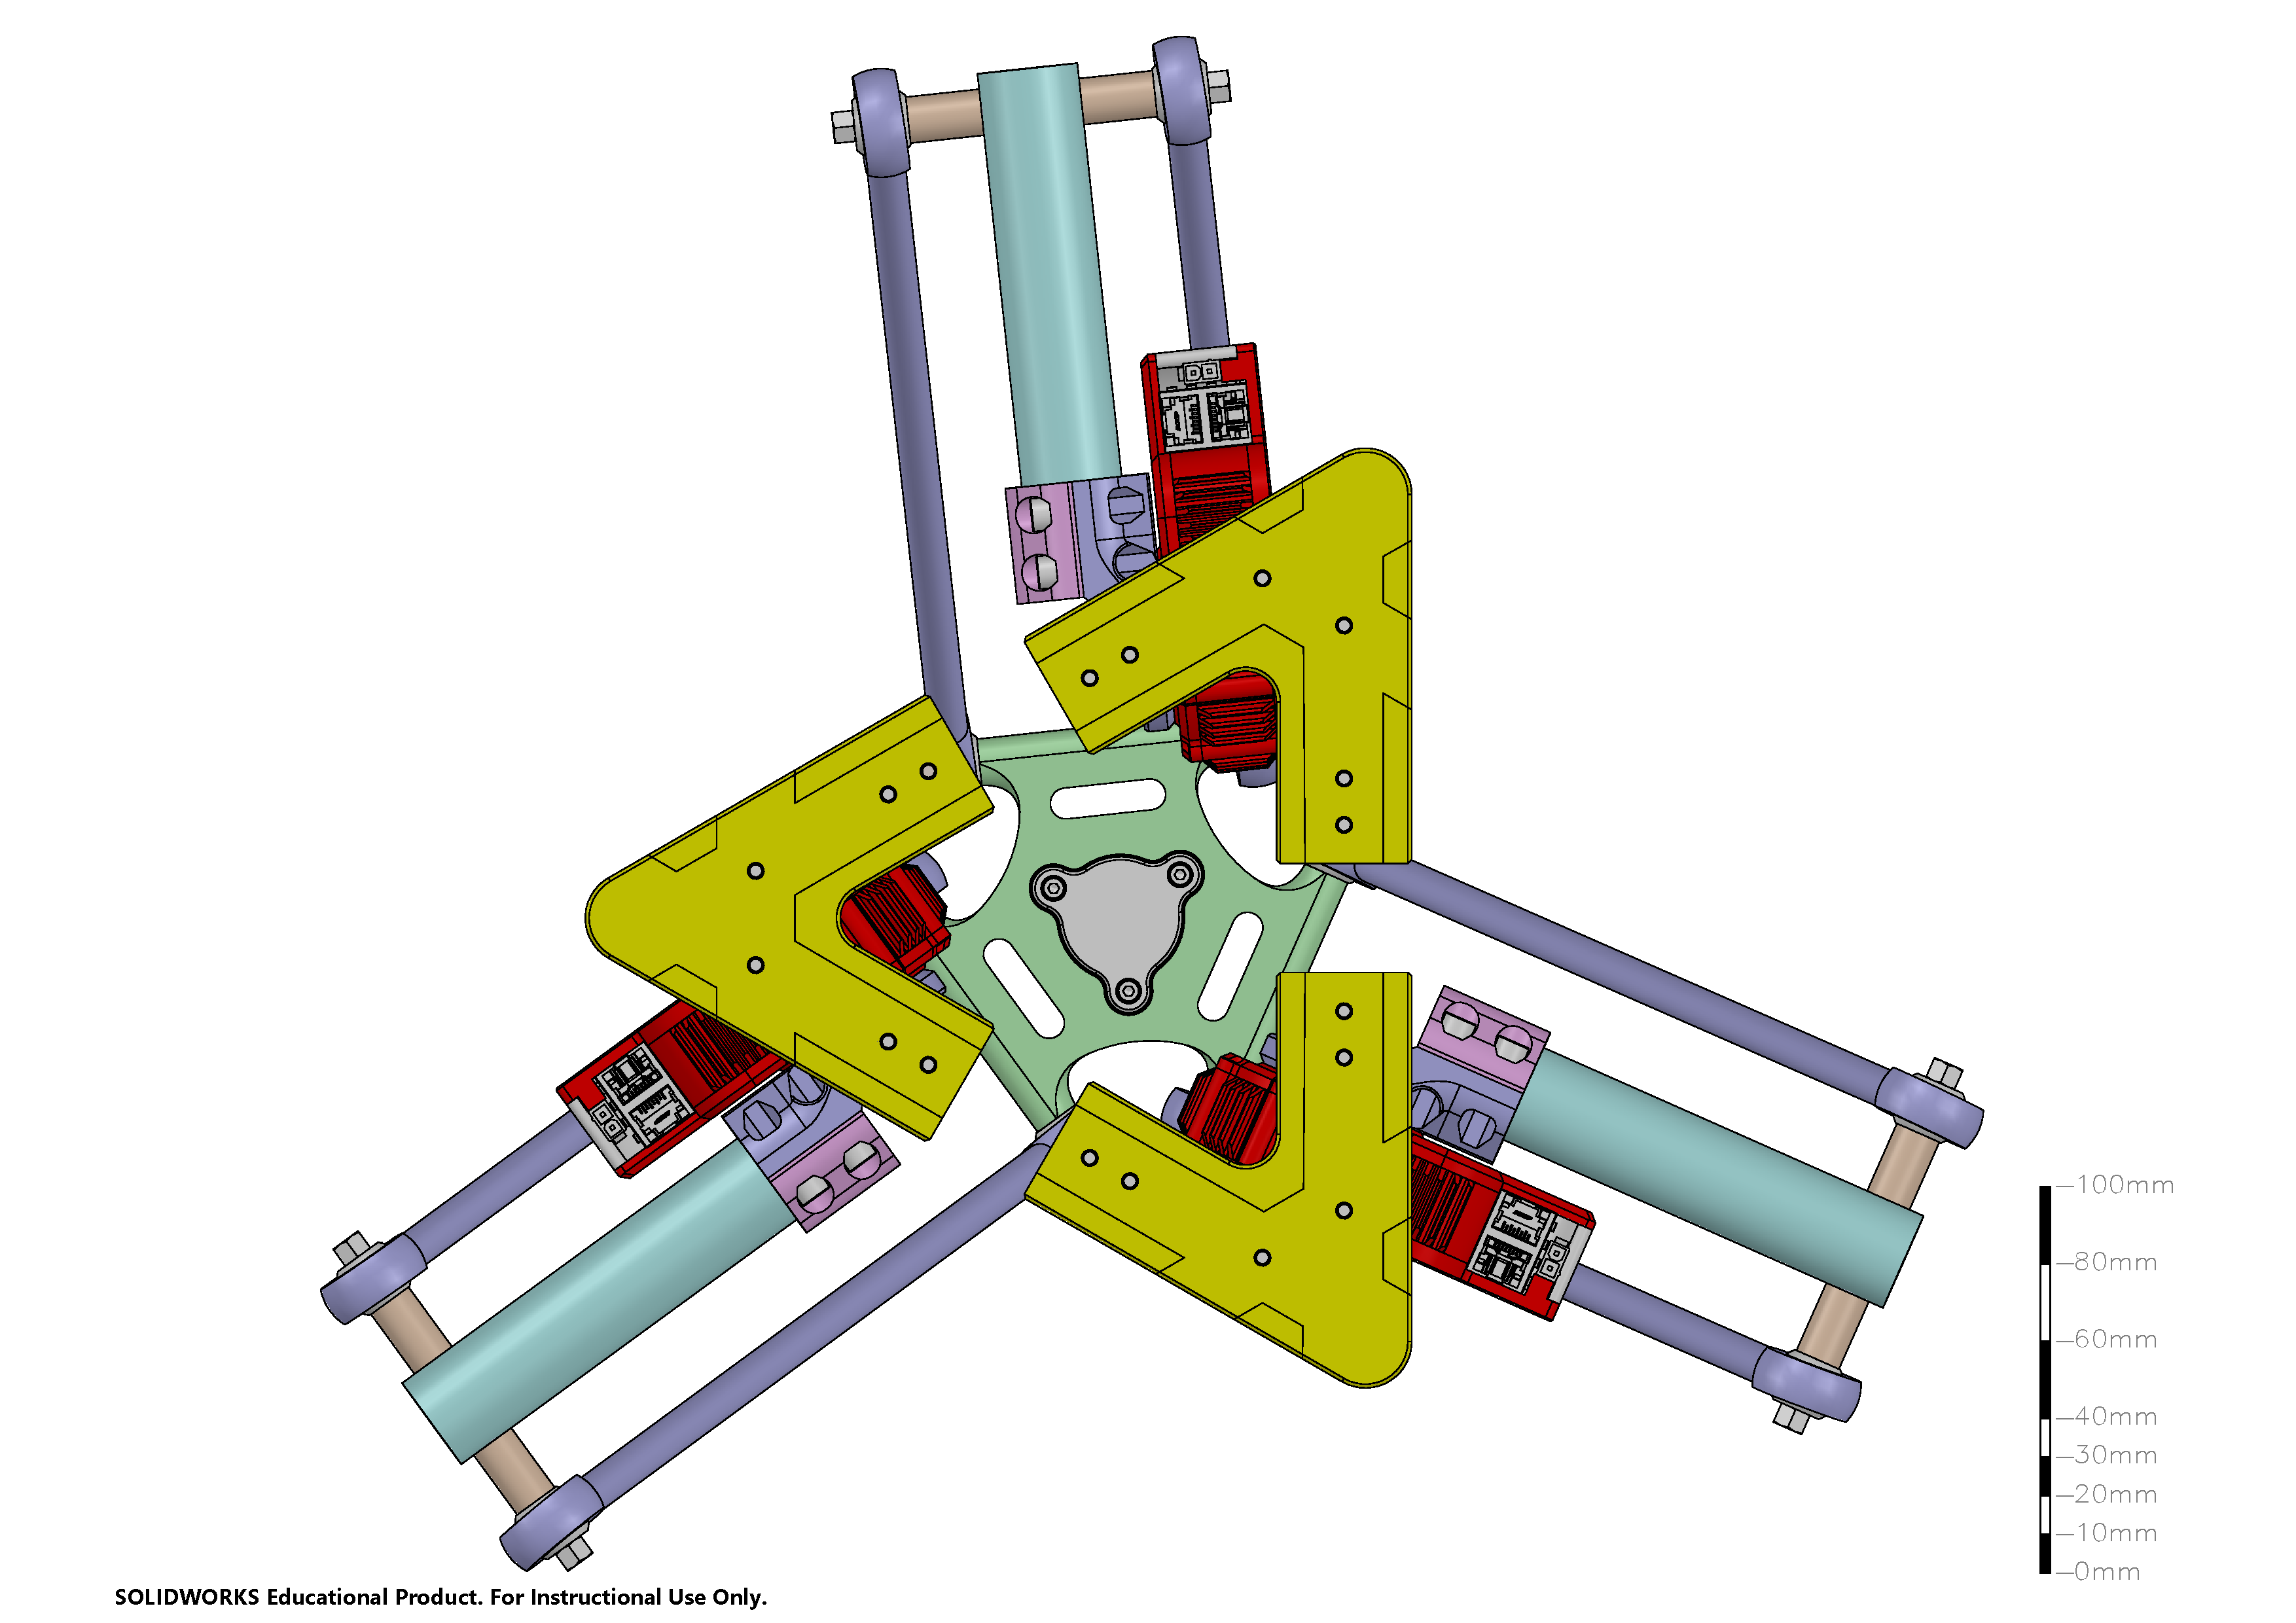
\includegraphics[width=\linewidth]{delta-unattached-top-view.PDF}
    %   \caption[Draufsicht des Delta-Roboters.]{Draufsicht des Delta-Roboters.}
    %   \label{fig:delta-unattached-top-view}
    % \end{figure}
    
\end{document}

%%%%%%%%%%%%%%%%%%%%%%%%%%%%%%%%%%%%%%%%%%%%%%%%%%%%
%%                     FIN                        %%
%%%%%%%%%%%%%%%%%%%%%%%%%%%%%%%%%%%%%%%%%%%%%%%%%%%%